% !TeX program = xelatex
% --- 1. FONT SIZE: 11pt (Strictly per Template) ---
\documentclass[11pt,a4paper]{report}

% =========================================================
% 1. DOCUMENT SETUP
% =========================================================

% --- 2. : 2.5cm on all sides (Strictly per Template) ---
\usepackage[margin=2.5cm, bindingoffset=0.8cm]{geometry}

% --- LINE SPACING: 1.5 (Strictly per Template) ---
\usepackage{setspace}
\onehalfspacing

% --- REQUIRED PACKAGES ---
\usepackage{pdfpages} % To insert Cover & Approval PDFs
\usepackage{tikz}
\usetikzlibrary{shapes.geometric, arrows, positioning, shadows}
\usepackage{pgfgantt}
\usepackage{graphicx}
\graphicspath{ {./images/} } 
\usepackage{float}       
\usepackage{booktabs}    
\usepackage{longtable}   
\usepackage{array}       
\usepackage{tabularx}    
\usepackage{enumitem}    
\usepackage[hidelinks]{hyperref} 
\usepackage{titlesec}
\usepackage{fancyhdr}

% --- Custom Columns & Lists ---
\newcolumntype{L}{>{\bfseries\raggedright\arraybackslash}p{3.5cm}} 
\newcolumntype{R}{>{\raggedright\arraybackslash}X} 
\newlist{normalsteps}{enumerate}{1}
\setlist[normalsteps,1]{nosep, leftmargin=*, label=\arabic*., before=\vspace{-0.5\baselineskip}, after=\vspace{0.6\baselineskip}}
\newlist{altsteps}{enumerate}{1}
\setlist[altsteps,1]{nosep, leftmargin=1.5em, label=\roman*., before=\vspace{0pt}, after=\vspace{0.3\baselineskip}}

% --- Fonts (Times New Roman) ---
\usepackage{fontspec}
\setmainfont{Times New Roman}[
Path = C:/Windows/Fonts/,
Extension = .ttf,
UprightFont = times,
BoldFont = timesbd,
ItalicFont = timesi,
BoldItalicFont = timesbi
]

% =========================================================
% 3. HEADING STYLES (Clean Chapter Page)
% =========================================================

% A. FOR NUMBERED CHAPTERS (Centers title on blank page)
\titleformat{name=\chapter}[display]
{\thispagestyle{empty}\vspace*{\fill}\normalfont\fontsize{14}{16}\bfseries\centering}
{\chaptertitlename\ \thechapter}
{10pt}
{\Large}
[\vspace*{\fill}\clearpage]

% B. FOR UNNUMBERED CHAPTERS (TOC, Lists) - Normal style
\titleformat{name=\chapter, numberless}[display]
{\normalfont\fontsize{14}{16}\bfseries\centering}
{} % no Chapter number here
{0pt}
{\Large}

% C. SECTION HEADINGS (Size 12 per Template)
\titleformat{\section}
{\normalfont\fontsize{12}{14}\bfseries}{\thesection}{1em}{}

\titleformat{\subsection}
{\normalfont\fontsize{12}{14}\bfseries}{\thesubsection}{1em}{}

\titleformat{\subsubsection}
{\normalfont\fontsize{12}{14}\bfseries}{\thesubsubsection}{1em}{}

% --- Footer ---
\pagestyle{fancy}
\fancyhf{}
\fancyfoot[C]{\thepage}
\renewcommand{\headrulewidth}{0pt}

% =========================================================
% 2. DOCUMENT START
% =========================================================
\begin{document}
	
	% --- 1. INSERT COVER PAGE ---
	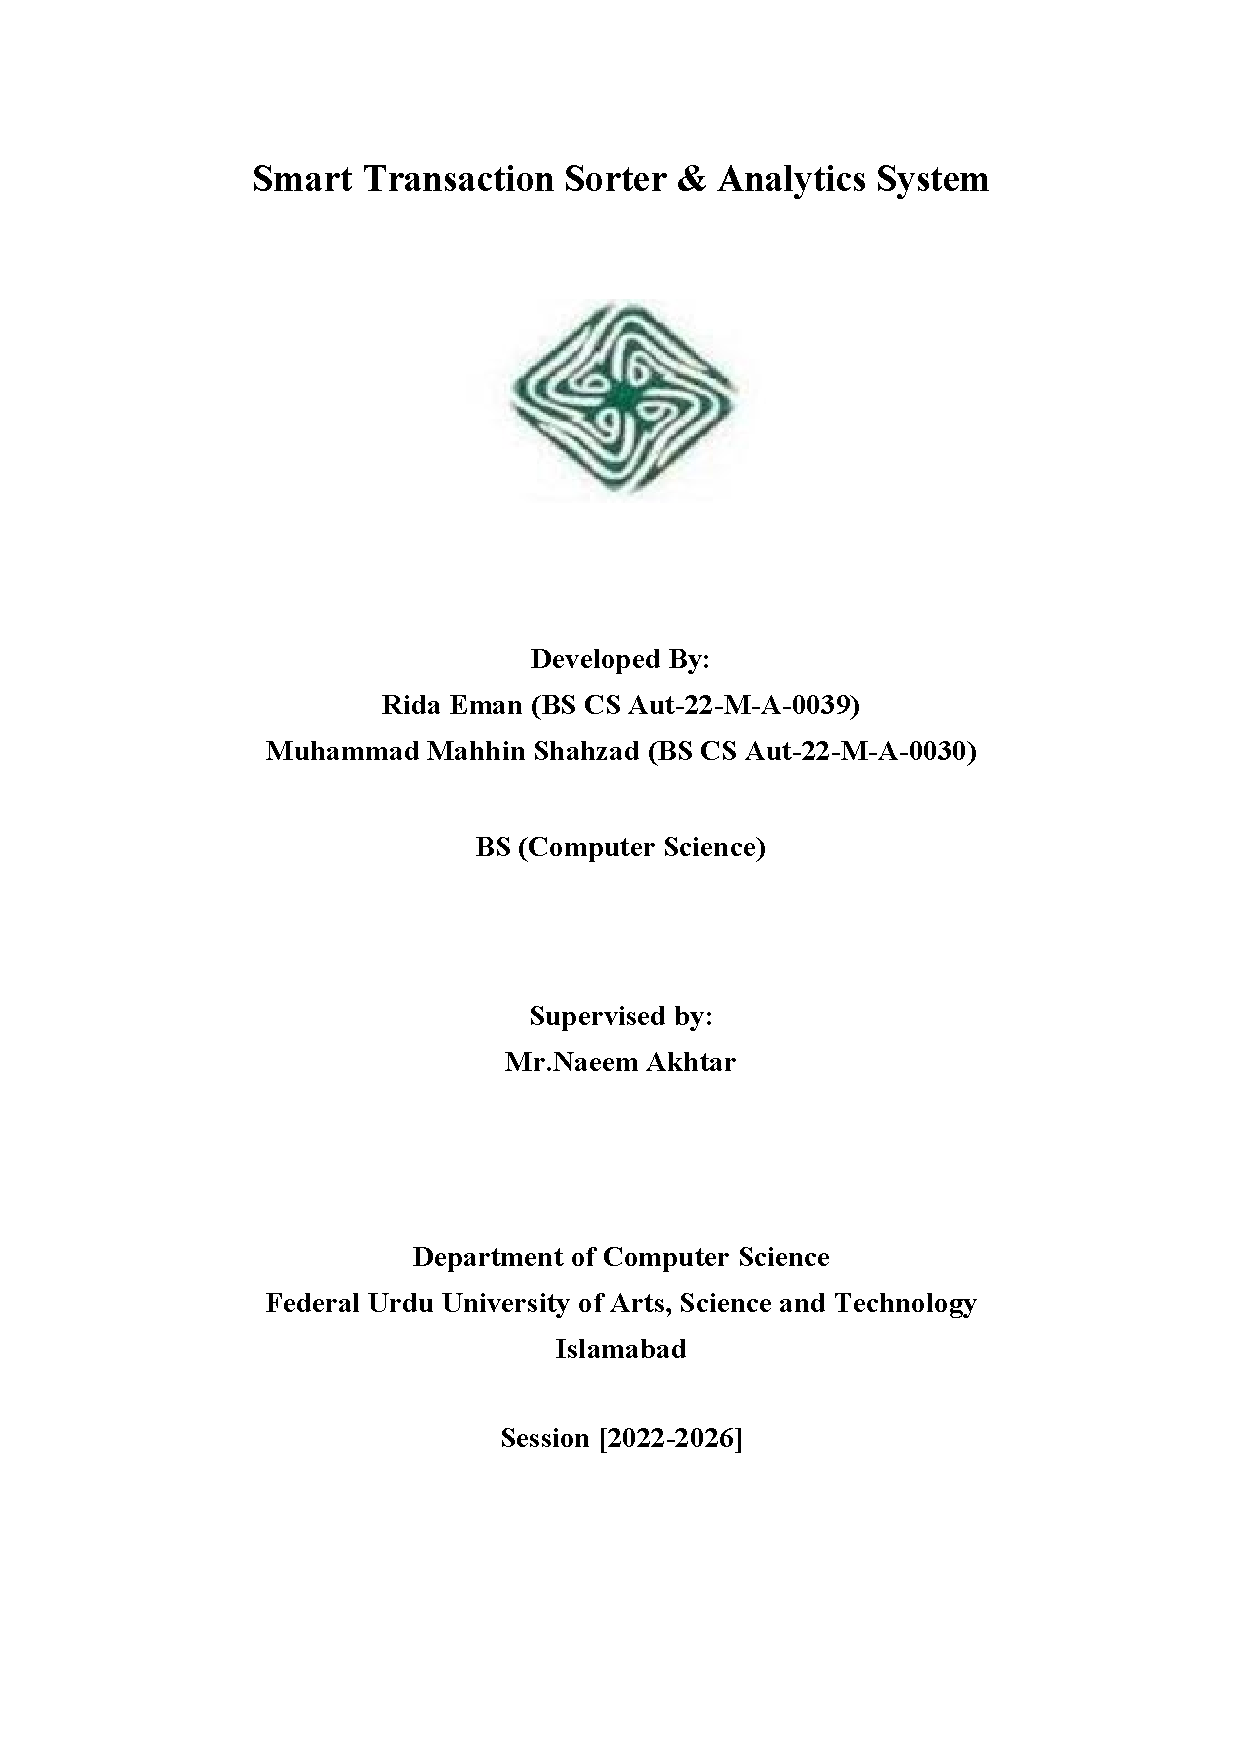
\includepdf[pages=-]{cover.pdf}
	
	% --- 2. INSERT APPROVAL PAGE ---
	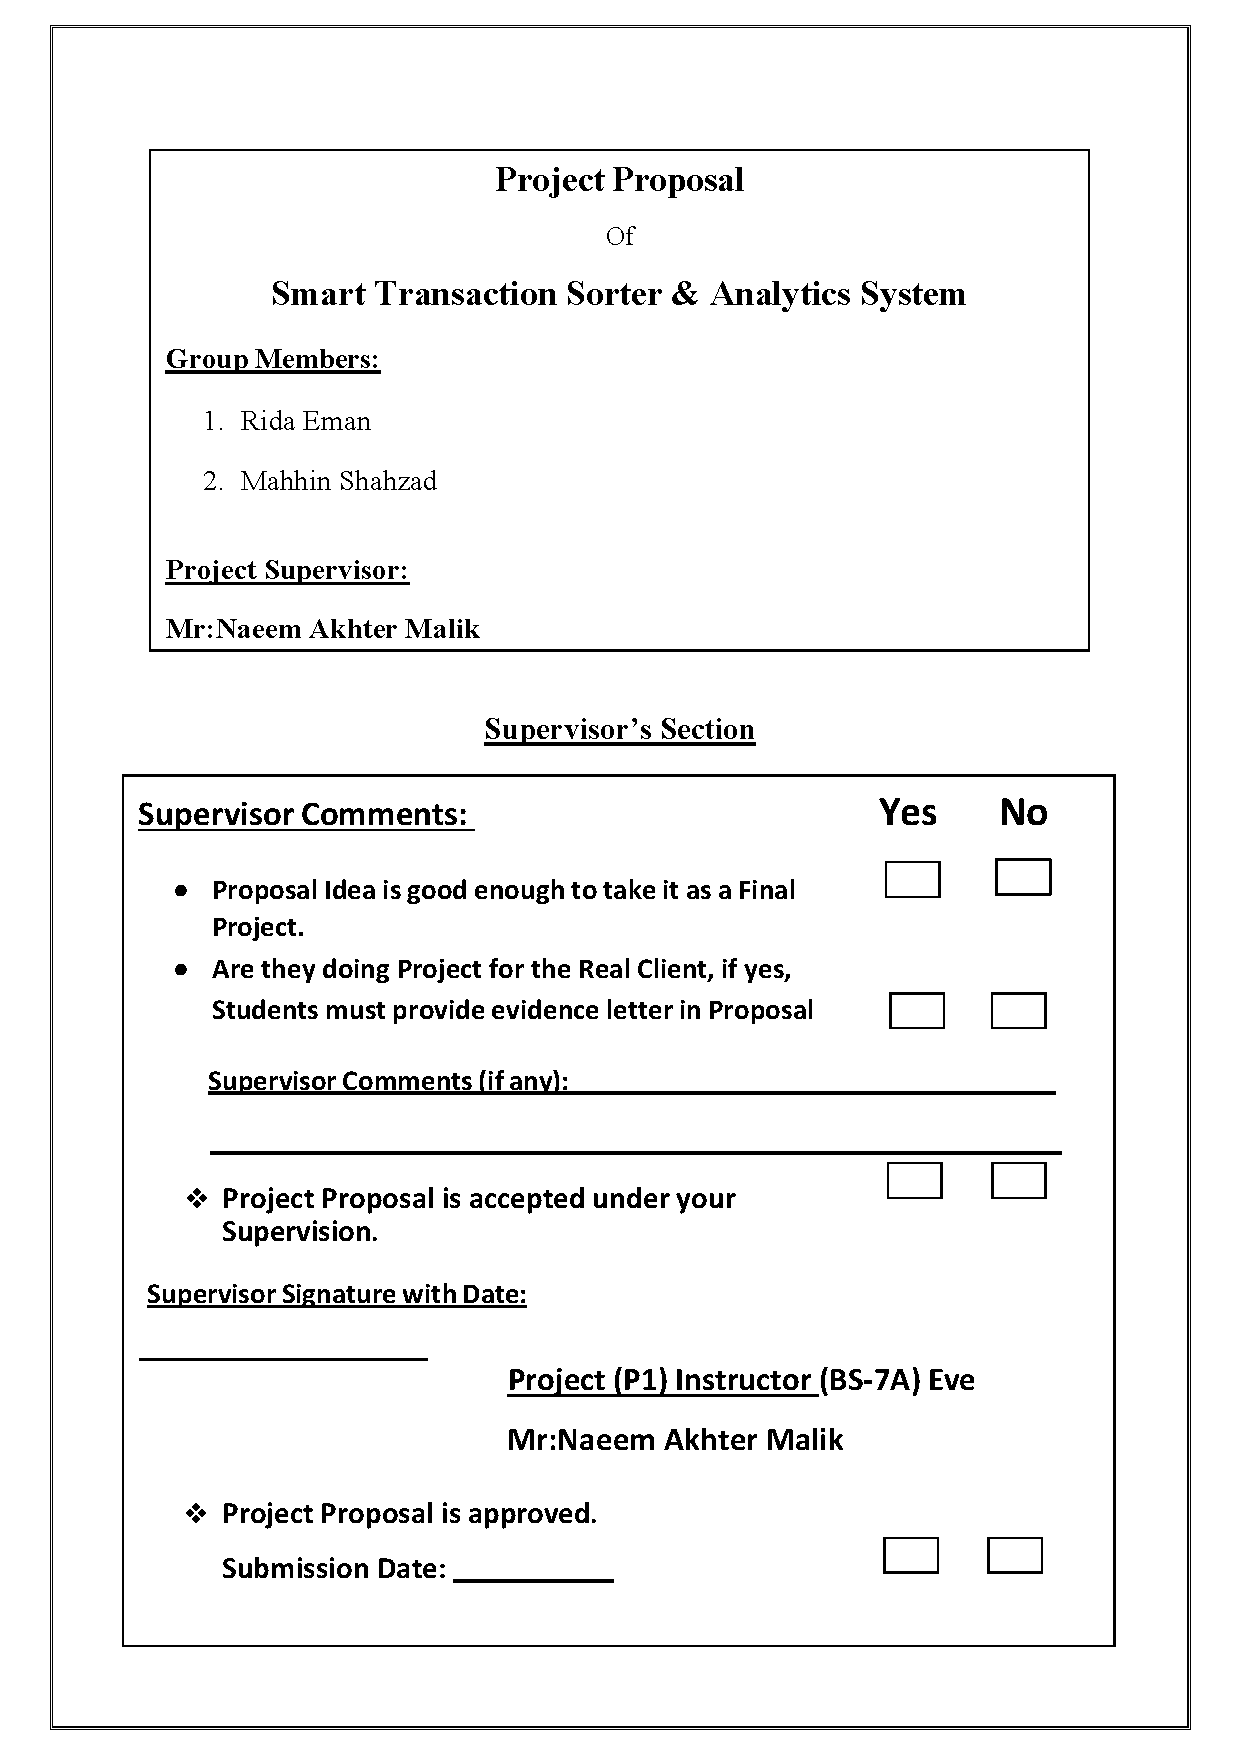
\includepdf[pages=-]{approval.pdf}
	
	% --- 3. Table of Contents ---
	\pagenumbering{roman} 
	\tableofcontents
	\newpage
	\listoffigures
	\newpage
	\pagenumbering{arabic}
	% =========================================================
% CHAPTER 1: INTRODUCTION                                                        \pagenumbering{arabic}
% =========================================================
% =========================================================
\chapter{Introduction}

\section{Introduction}
The rise of the digital economy in Pakistan has been driven by the widespread adoption of fintech platforms such as Easypaisa, SadaPay, and JazzCash. These services have empowered millions of users by simplifying payments and providing instant access to their complete transaction history. This readily available data holds the potential to offer valuable insights into personal spending habits. However, for most users, this potential remains untapped as the data is typically provided in raw formats (e.g., CSV files) without sophisticated analytical tools.

This proposal introduces the Smart Transaction Sorter and Analytics system, a web-based application designed to unlock the value hidden within this raw financial data. The project's academic objective is to develop a functional, standalone tool that serves as a research-based feasibility study. The resulting application will be architected as a powerful blueprint for an intelligent analytics module. The long-term vision, while outside the immediate scope of this project, is that such a module could be pitched for integration into the very fintech platforms it complements, thereby closing the significant analytical gap in the current market.

\section{Problem Statement}
The problem is the absence of an integrated Business Intelligence (BI) and analytics layer in Pakistan digital wallets. People export their data, move it into another tool, and tag each transaction by hand. It’s a manual and time-consuming process.

\section{Proposed System}
The proposed system is a standalone, web-based application focused on delivering a complete workflow from raw CSV data to a finalized BI dashboard. To automate data preparation for the dashboard, an intelligent sorting component leveraging a pre-trained language model capable of contextual understanding will be included. The system aims to demonstrate feasibility using publicly available, realistic transaction data. The core functionality is broken down as follows:

\begin{enumerate}
	\item \textbf{Custom Category Management:} The user will first define their own set of personal spending categories (e.g., Groceries, Transport, Health \& Fitness).
	\item \textbf{CSV Data Ingestion:} The user then uploads their transaction history as a standard CSV file. This serves as the primary data input mechanism.
	\item \textbf{Intelligent Sorting Component:} A smart classification component, utilizing the pre-trained language model, will process the raw data. It will analyze transaction descriptions and human-like notes/comments, mapping each entry to the most relevant category from the user's own custom list. This automated step moves beyond simple rule-based mapping to understand context, preparing the data accurately for the BI layer.
	\item \textbf{Interactive BI Visualization:} Once sorted, the data is presented to the user through an interactive Business Intelligence (BI) dashboard. This dashboard is the primary output and will feature charts and graphs visualizing spending breakdowns tailored to the user's personal financial structure.
	\item \textbf{Validation with Public Data:} To demonstrate the effectiveness and real-world applicability of the sorting component, the system will be tested and validated using a relevant public dataset. This dataset will contain transaction-like entries with descriptions and comments, allowing for rigorous evaluation of the classification accuracy without relying on proprietary user data.
\end{enumerate}
By leveraging a sorting mechanism powered by a pre-trained language model, adaptable to user categories and validated on public data, the application will deliver personalized and accurate insights through its core BI and visualization dashboard.

\section{Survey of the Related Applications}
To establish the necessity of this project, this survey analyzes two distinct application categories: the local digital wallets that create the data and the problem, and the global expense trackers that represent existing but flawed solutions.

\subsection{A. Market Survey — Local Digital Wallets (Direct Context)}
A review of the official documentation for Pakistan's leading digital wallets confirms that while they excel at payments, they generally lack a mature, integrated analytics tool.
\begin{itemize}
	\item \textbf{SadaPay, NayaPay, \& Easypaisa:} These platforms reliably provide users with the ability to download their account statements or view transaction histories, with some confirming CSV export availability. However, their feature sets do not include built-in BI or smart analytics layers.
	\item \textbf{JazzCash:} While also providing standard statements, JazzCash recently announced a Spending Tracker feature. Based on its public introduction, this appears to be a basic tracking tool for monitoring budgets. While a positive step, it is distinct from a full-scale BI layer and does not offer the intelligent, personalized categorization that is central to this proposal.
\end{itemize}
\textit{Implication.} The local market either offers no native analytics or, at best, provides basic tracking. This creates a clear analytics vacuum and validates the need for a separate application to provide the missing intelligence.

\subsection{B. Indirect Comparators — Global CSV-Import Tools}
Global platforms like YNAB and Mint demonstrate the feasibility of the CSV-import workflow but are poorly suited to the local context and fail to solve the core problem of personalization.
\begin{itemize}
	\item \textbf{High-Friction Workflow:} Tools like YNAB and Mint, while powerful, still require significant manual effort after a CSV import to clean up data and assign categories line-by-line. This does not solve the primary issue of laborious manual work.
	\item \textbf{Lack of Personalization and Intelligence:} These platforms are separate, often paid services that use rigid, generic categorization systems. They lack the intelligent sorting component needed to learn and adapt to a user's own custom financial categories, failing the key protein bar test case.
	\item \textbf{Misaligned Business Model:} Their primary model is direct bank API integration, which is not the standard in the Pakistani market. Their CSV import tools are a secondary feature, not the core product.
\end{itemize}
\textit{Implication.} The global tools prove the CSV-to-analytics model is viable but highlight a gap for a more intelligent, low-friction, and personalized solution tailored to the realities of the local market. This project is designed specifically to fill that gap.

\section{Modules \& Sub-modules}
The system architecture will be broken down into the following modules and sub-modules to ensure a clear separation of concerns and facilitate iterative development.

\subsection{User \& Category Management Module}
This module will handle all user-facing administrative tasks and personalization features.
\begin{itemize}
	\item \textbf{Authentication Submodule:} This submodule is responsible for secure user registration, login, logout, and session management to ensure data privacy.
	\item \textbf{Category CRUD Submodule:} This provides the interface and backend logic for users to Create, Read, Update, and Delete (CRUD) their personalized list of spending categories.
\end{itemize}

\subsection{Data Ingestion Module}
This module serves as the primary data entry point for transaction histories.
\begin{itemize}
	\item \textbf{File Upload Submodule:} This submodule provides the secure, user-facing web form for uploading transaction data in CSV format.
	\item \textbf{CSV Validation Submodule:} This is a backend service that parses the uploaded file and verifies its structural integrity, ensuring required columns (e.g., Date, Description, Amount) are present.
\end{itemize}

\subsection{Intelligent Sorting Module}
This module contains the core data processing and classification logic.
\begin{itemize}
	\item \textbf{Data Pre-processing Submodule:} This submodule cleans and standardizes the validated data, converting data types (e.g., string dates to date objects) to prepare it for classification.
	\item \textbf{Classification Engine Submodule:} This is the smart component that takes a transaction's text and the user's custom category list as input, and outputs the most probable category.
	\item \textbf{Database Persistence Submodule:} This submodule saves the processed transaction data, along with its newly assigned category, into the database.
\end{itemize}

\subsection{BI \& Visualization Module}
This module is responsible for presenting the final analytical output to the user.
\begin{itemize}
	\item \textbf{Data Aggregation Submodule:} This is a backend service that runs queries on the database to aggregate data for visualization (e.g., calculating total spending per category).
	\item \textbf{Dashboard Rendering Submodule:} This is the frontend component that takes the aggregated data and uses a charting library to render the interactive BI dashboard.
\end{itemize}

\section{Primary Actors}
The system is designed for a single primary actor:
\begin{itemize}
	\item \textbf{The User:} An individual who wants to analyze their personal financial transaction history. The User will be able to perform the following actions:
	\begin{itemize}
		\item Register for an account and log in securely.
		\item Create and manage their own personalized list of spending categories.
		\item Upload their transaction history in CSV format.
		\item View the interactive BI dashboard with visualizations of their spending.
		\item (Optional) Review and manually correct any automated classifications.
	\end{itemize}
\end{itemize}

\section{Tools \& Techniques}
The project will be developed using a modern, robust technology stack to ensure scalability and maintainability.
\begin{itemize}
	\item \textbf{Backend Framework:} Python with the Django Framework will be used to build the server-side logic, manage URLs, and handle database interactions.
	\item \textbf{Database:} SQLite will be used for development due to its simplicity. The system will be designed to be compatible with PostgreSQL for potential production deployment.
	\item \textbf{Data Processing:} The Pandas library will be used for efficient parsing, validation, and manipulation of the uploaded CSV data.
	\item \textbf{Intelligent Sorting:} The Hugging Face \texttt{Transformers} library will be utilized to implement the classification component, leveraging a pre-trained zero-shot classification model).
	\item \textbf{Frontend Visualization:} A JavaScript library such as Plotly.js or Chart.js will be used to render the interactive charts and graphs on the BI dashboard.
	\item \textbf{Web Technologies:} The user interface will be built with standard HTML, CSS, and JavaScript.
\end{itemize}

\section{Process Model \& Design Approach}
The project will be developed using an Iterative and Incremental process model. This approach is well-suited for a modular system, as it allows for the development and testing of each component in successive cycles or iterations.

The development will proceed by building and testing each module individually before integrating them into a cohesive whole. This allows for early feedback, easier debugging, and a more manageable workflow. The design approach will follow the Model-View-Template (MVT) architectural pattern, which is native to the Django framework and provides a clear separation between data logic, business logic, and user interface.

\section{Project Plan}
The project timeline is scheduled over approximately seven months (30 weeks), visualized in the Gantt chart in Figure \ref{fig:gantt} below. The plan prioritizes documentation and core feature development first, followed by the integration of the intelligent sorting component and finalization.

\begin{figure}[H]
	\centering
	\resizebox{\textwidth}{!}{
		\begin{ganttchart}[
			vgrid,
			hgrid,
			bar/.append style={fill=blue!50},
			milestone/.append style={fill=red!70}
			]{1}{30}
			\gantttitle{Project Timeline (Weeks)}{30} \\
			\gantttitlelist{1,...,30}{1} \\
			
			% Phase 1: Documentation & Initial Setup
			\ganttgroup{Phase 1: Planning \& Design}{1}{8} \\
			\ganttmilestone[name=p1]{Proposal Submission}{1} \ganttnewline
			\ganttlinkedbar[name=srs]{SRS Documentation}{2}{3} \ganttnewline
			\ganttlinkedbar[name=uc]{Use Case Diagrams}{3}{5} \ganttnewline
			\ganttlinkedbar[name=ui]{Initial UI/UX Design}{5}{8} \ganttnewline
			
			% Phase 2: Core CSV & BI Development
			\ganttgroup{Phase 2: Core Feature Development}{9}{18} \\
			\ganttlinkedbar[name=data]{Develop Data Ingestion (CSV)}{9}{12} \ganttnewline
			\ganttlinkedbar[name=db]{Database \& Backend Setup}{11}{14} \ganttnewline
			\ganttlinkedbar[name=bi]{Develop BI \& Visualization Module}{13}{18} \ganttnewline
			
			% Phase 3: AI Integration & Testing
			\ganttgroup{Phase 3: AI Integration}{19}{25} \\
			\ganttlinkedbar[name=ai]{Develop Intelligent Sorting Module}{19}{22} \ganttnewline
			\ganttlinkedbar[name=integ]{Integrate Sorting with Main App}{23}{25} \ganttnewline
			
			% Phase 4: Finalization & Reporting
			\ganttgroup{Phase 4: Finalization \& Reporting}{26}{30} \\
			\ganttlinkedbar[name=test]{End-to-End Testing \& Bug Fixing}{26}{28} \ganttnewline
			\ganttlinkedbar[name=doc]{Final Report Documentation}{28}{29} \ganttnewline
			\ganttmilestone[name=p2]{Final Presentation}{30}
			
			% Links
			\ganttlink{p1}{srs}
			\ganttlink{srs}{uc}
			\ganttlink{uc}{ui}
			\ganttlink{ui}{data}
			\ganttlink{data}{db}
			\ganttlink{db}{bi}
			\ganttlink{bi}{ai}
			\ganttlink{ai}{integ}
			\ganttlink{integ}{test}
			\ganttlink{test}{doc}
			\ganttlink{doc}{p2}
		\end{ganttchart}
	}
	\caption{Project development timeline presented as a Gantt chart.}
	\label{fig:gantt}
\end{figure}
% =========================================================
% CHAPTER 2: REQUIREMENTS SPECIFICATION
% =========================================================
\chapter{Requirements Specification}

\section{Purpose}
The purpose of the Smart Transaction Sorter and Analytics System is to provide users with an intelligent, automated way to analyze their personal financial spending. This web application uses Artificial Intelligence (AI) to categorize raw transaction data (from CSV files) and instantly convert it into clear, visual charts, eliminating the need for hours of frustrating manual work.

\section{Project Scope}
The scope of this project is a standalone, web-based tool that accepts a financial history file (CSV), uses AI to categorize every line based on user-defined labels, and presents the results on a BI Dashboard. The system includes User authentication, Category Management, CSV Upload/Validation, AI Sorting Logic, Data Persistence, and a Visualization Dashboard.

\begin{itemize}
	\item \textbf{In Scope:} User login, Category creation, CSV parsing, AI classification, Dashboard charts.
	\item \textbf{Out of Scope:} Direct integration (API) with bank/wallet accounts, payment processing, or real-time transaction tracking.
\end{itemize}

\section{Definitions, Acronyms, and Abbreviations}
\renewcommand{\arraystretch}{1.5}
\begin{longtable}{|p{4cm}|p{10.5cm}|}
	\hline
	\textbf{Term/Abbreviation} & \textbf{Definition} \\
	\hline
	\endfirsthead
	\hline
	\textbf{Term/Abbreviation} & \textbf{Definition} \\
	\hline
	\endhead
	STS & Smart Transaction Sorter (The name of this application). \\ \hline
	AI & Artificial Intelligence (The component that performs automatic classification). \\ \hline
	CSV & Comma-Separated Values (The standard file format for data input/upload). \\ \hline
	BI & Business Intelligence (Refers to the analytical dashboard and visualization tools). \\ \hline
	DB & Database (The system storage where user and financial data are saved). \\ \hline
\end{longtable}

\section{Document Overview}
This document describes the requirements for the Smart Transaction Sorter and Analytics System (STS). It serves as the single reference point for what the system must do and how well it must perform. The STS acts as a complimentary Business Intelligence layer for existing digital wallets and bank applications that currently only offer raw data exports.

\section{Functional Requirements}

\subsection{Security Management}

\subsubsection{Process Sign Up}
\begin{longtable}{|p{2.5cm}|p{12cm}|}
	\hline
	\textbf{ID} & \textbf{Requirement Description} \\
	\hline
	SRS-1 & The system shall allow new users to securely register by providing a username, email, and password. \\ \hline
	SRS-2 & The system must validate that the email address is unique and not already registered. \\ \hline
	SRS-3 & The system shall store user passwords using a strong one-way hash (never in plain text). \\ \hline
	SRS-4 & Upon successful registration, the system shall create a dedicated, isolated database scope for the user. \\ \hline
\end{longtable}

\subsubsection{Process Sign In / Logout}
\begin{longtable}{|p{2.5cm}|p{12cm}|}
	\hline
	\textbf{ID} & \textbf{Requirement Description} \\
	\hline
	SRS-5 & The system shall allow registered users to log in securely using their credentials. \\ \hline
	SRS-6 & The system shall use HTTPS/SSL for all data transfer between the client and server to prevent interception. \\ \hline
	SRS-7 & The system shall allow users to securely log out, terminating their current session. \\ \hline
\end{longtable}

\subsection{Category Management}

\subsubsection{Create Spending Category}
\begin{longtable}{|p{2.5cm}|p{12cm}|}
	\hline
	\textbf{ID} & \textbf{Requirement Description} \\
	\hline
	SRS-8 & The system shall allow users to create new, personalized spending category labels (e.g., "Groceries", "Utilities"). \\ \hline
	SRS-9 & The system shall validate that the category name is not a duplicate within the user's profile. \\ \hline
	SRS-10 & The system shall ensure all created categories are immediately available for the AI Sorting Engine to use. \\ \hline
\end{longtable}

\subsubsection{Manage Spending Categories}
\begin{longtable}{|p{2.5cm}|p{12cm}|}
	\hline
	\textbf{ID} & \textbf{Requirement Description} \\
	\hline
	SRS-11 & The system shall allow users to view a list of all their existing categories. \\ \hline
	SRS-12 & The system shall allow users to edit the name of an existing category. \\ \hline
	SRS-13 & The system shall allow users to delete a category (and optionally reassign its associated transactions). \\ \hline
\end{longtable}

\subsection{Data Ingestion Management}

\subsubsection{Upload Transaction File (CSV)}
\begin{longtable}{|p{2.5cm}|p{12cm}|}
	\hline
	\textbf{ID} & \textbf{Requirement Description} \\
	\hline
	SRS-14 & The system shall provide a simple interface for the user to upload a transaction history file. \\ \hline
	SRS-15 & The system is constrained to accepting only CSV (Comma-Separated Values) file formats. \\ \hline
	SRS-16 & The system shall provide a progress indicator or status feedback during the upload process. \\ \hline
\end{longtable}

\subsubsection{File Validation}
\begin{longtable}{|p{2.5cm}|p{12cm}|}
	\hline
	\textbf{ID} & \textbf{Requirement Description} \\
	\hline
	SRS-17 & The system shall check the uploaded file for necessary columns (specifically: Date, Description, and Amount). \\ \hline
	SRS-18 & The system shall provide clear, user-friendly error messages if the file structure is invalid or missing data. \\ \hline
	SRS-19 & The system shall reject files that exceed a predefined size limit to maintain performance. \\ \hline
\end{longtable}

\subsection{Intelligent Sorting Management}

\subsubsection{Process Transactions (AI Sorting)}
\begin{longtable}{|p{2.5cm}|p{12cm}|}
	\hline
	\textbf{ID} & \textbf{Requirement Description} \\
	\hline
	SRS-20 & The system shall use a smart classification model (AI) to read transaction descriptions from the uploaded file. \\ \hline
	SRS-21 & The system shall automatically assign the most relevant custom category to each transaction. \\ \hline
	SRS-22 & The system shall utilize the Hugging Face Transformers library for the classification logic. \\ \hline
\end{longtable}

\subsubsection{Data Persistence \& Saving}
\begin{longtable}{|p{2.5cm}|p{12cm}|}
	\hline
	\textbf{ID} & \textbf{Requirement Description} \\
	\hline
	SRS-23 & The system shall securely save the processed transaction data, including the new category label, to the user's database. \\ \hline
	SRS-24 & The system shall ensure that once categorized, the financial history persists until explicitly deleted by the user. \\ \hline
\end{longtable}

\subsection{Analytics Management}

\subsubsection{View Dashboard}
\begin{longtable}{|p{2.5cm}|p{12cm}|}
	\hline
	\textbf{ID} & \textbf{Requirement Description} \\
	\hline
	SRS-25 & The system shall display a primary BI (Business Intelligence) dashboard view after processing is complete. \\ \hline
	SRS-26 & The dashboard shall be interactive, allowing users to hover over elements for more details. \\ \hline
\end{longtable}

\subsubsection{View Spending Breakdown}
\begin{longtable}{|p{2.5cm}|p{12cm}|}
	\hline
	\textbf{ID} & \textbf{Requirement Description} \\
	\hline
	SRS-27 & The system shall display clear charts (e.g., pie charts) visualizing total spending broken down by custom categories. \\ \hline
	SRS-28 & The system shall calculate and display total expenditure for the uploaded period. \\ \hline
\end{longtable}

\subsection{Administrator Management}

\subsubsection{Admin Panel Access}
\begin{longtable}{|p{2.5cm}|p{12cm}|}
	\hline
	\textbf{ID} & \textbf{Requirement Description} \\
	\hline
	SRS-29 & The System Administrator must use distinct credentials to log in to the dedicated administrative interface. \\ \hline
	SRS-30 & The Admin Panel shall be secured and inaccessible to standard users. \\ \hline
\end{longtable}

\subsubsection{User Account Management}
\begin{longtable}{|p{2.5cm}|p{12cm}|}
	\hline
	\textbf{ID} & \textbf{Requirement Description} \\
	\hline
	SRS-31 & The Admin shall have the ability to View and Search for any registered user account. \\ \hline
	SRS-32 & The Admin shall have the ability to Create, Edit, or Delete user accounts if necessary. \\ \hline
	SRS-33 & The Admin shall have read-only access to view user-created Categories and processed Transactions for auditing purposes. \\ \hline
\end{longtable}

\section{Non-Functional Requirements}

\subsection{Security}
\begin{itemize}
	\item \textbf{Account Protection:} User passwords must be stored using a strong one-way hash.
	\item \textbf{Session Security:} The system must use HTTPS for all communication to prevent data interception.
	\item \textbf{User Isolation:} A user's data must be completely isolated and inaccessible to any other user.
\end{itemize}

\subsection{Usability}
\begin{itemize}
	\item The interface must be intuitive, clean, and fully mobile-responsive.
	\item Training time for a normal user to understand the upload and sort process should be minimal (intuitive design).
\end{itemize}

\subsection{Reliability}
\begin{itemize}
	\item The system must be available and function correctly 99.5\% of the time.
	\item In any error scenario, the system must provide an appropriate message and retain the state of the user's data (no silent failures).
\end{itemize}

\subsection{Performance}
\begin{itemize}
	\item \textbf{File Processing Time:} A standard file (up to 500 transactions) must be processed, sorted by the AI, and ready for viewing within 60 seconds.
	\item The system dashboard should load visualization results in under 3 seconds after processing is complete.
\end{itemize}

\subsection{Design Constraints}
\begin{itemize}
	\item \textbf{Technology Stack:} Must use Python (Django Framework) for the backend logic.
	\item \textbf{Database:} Designed for use with PostgreSQL for scalability.
	\item \textbf{AI Library:} The system must utilize the Hugging Face Transformers library.
	\item \textbf{Architecture:} The code must follow the MVT (Model-View-Template) architectural pattern.
\end{itemize}

\subsection{Data Ownership \& Business Rules}
\begin{itemize}
	\item \textbf{Data Ownership:} All uploaded data remains the intellectual property of the User.
	\item \textbf{No Third-Party Sharing:} User financial data may not be shared, sold, or exposed to any third party.
	\item \textbf{Persistence:} Processed data remains available until the user explicitly decides to delete it.
\end{itemize}

\section{External Interface Requirements}

\subsection{User Interfaces}
The user interface will be entirely web-based, optimized for responsive viewing on desktop and mobile devices. Key interfaces include:
\begin{itemize}
	\item Login/Registration Forms.
	\item Custom Category Management Form (CRUD interface).
	\item CSV File Upload Interface with progress/status feedback.
	\item Interactive BI Dashboard (using modern charting libraries like Plotly.js or Chart.js).
	\item A secure Admin Panel (for System Administrator use only).
\end{itemize}

\subsection{Hardware Interfaces}
No specialized hardware is required. The system will interface with standard internet-supported client devices (PC, laptop, mobile, tablet).

\subsection{Software Interfaces}
The system interfaces with the following software components:
\begin{itemize}
	\item \textbf{Python / Django:} Primary backend web application and API interface.
	\item \textbf{PostgreSQL:} Database management system for data persistence.
	\item \textbf{Pandas Library:} Used for data manipulation, CSV parsing, and validation.
	\item \textbf{Hugging Face Transformers:} The core library used for the AI classification model.
	\item \textbf{Plotly.js / Chart.js:} Frontend JavaScript libraries for rendering visualizations.
\end{itemize}

% =========================================================
% CHAPTER 3: USE CASE ANALYSIS
% =========================================================
\chapter{Use Case Analysis}


\section{Use Case Diagram}
The Use Case Diagram provides a high-level overview of the system's interactions with the primary actors (User and System Administrator).

\begin{figure}[H]
	\centering
	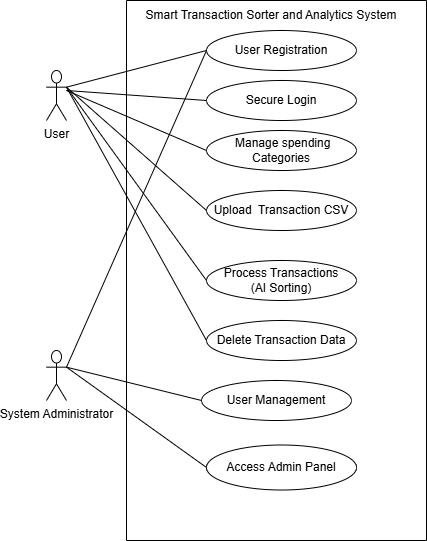
\includegraphics[width=0.9\textwidth, height=13cm, keepaspectratio]{usecase_diagram.png}
	\caption{Smart Transaction Sorter System Use Case Diagram}
	\label{fig:usecase_diagram}
\end{figure}

\section{Fully Dressed Use Case Scenarios}

\subsection{User Access \& Authentication}

% --- USE CASE 1.1 ---
\subsubsection{Use Case 1.1: User Registration}
\begin{tabularx}{\textwidth}{|L|R|}
	\hline
	Use Case ID & 1.1 \\ \hline
	Use Case Name & User Registration \\ \hline
	Actor & User \\ \hline
	Description & A new user creates a secure account to access the system features. \\ \hline
	Preconditions & User has a valid email address and internet access. \\ \hline
	Postconditions & A new user account is created in the database, and the user is redirected to the login page. \\ \hline
	Priority & High \\ \hline
	Normal Course & 
	\begin{normalsteps}
		\item User navigates to the application landing page.
		\item User selects "Register".
		\item System displays the registration form.
		\item User enters Name, Email, and Password (twice).
		\item System validates the input format.
		\item System hashes the password and saves the new user record.
		\item System displays a success message.
	\end{normalsteps} \\ \hline
	Alternative Courses & 
	\textbf{5a. Weak Password:} 
	\begin{altsteps}
		\item System detects password does not meet security complexity requirements.
		\item System prompts user to choose a stronger password.
	\end{altsteps} 
	\textbf{6a. Email Already Exists:} 
	\begin{altsteps}
		\item Database check confirms the email is already registered.
		\item System displays error: "Account already exists".
		\item System prompts user for Login.
	\end{altsteps} \\ \hline
	Exceptions & Database connection failure prevents account creation. \\ \hline
	Special Req. & Passwords must be hashed using a strong algorithm (e.g., PBKDF2 or Argon2) before storage. \\ \hline
\end{tabularx}

\newpage

% --- USE CASE 1.2 ---
\subsubsection{Use Case 1.2: Secure Login}
\begin{tabularx}{\textwidth}{|L|R|}
	\hline
	Use Case ID & 1.2 \\ \hline
	Use Case Name & Secure Login \\ \hline
	Actor & User, System Administrator \\ \hline
	Description & Users or Admins log in to access their respective dashboards. \\ \hline
	Preconditions & User/Admin must have a registered account. \\ \hline
	Postconditions & Actor is authenticated, a session is established, and they are redirected to their authorized dashboard. \\ \hline
	Priority & High \\ \hline
	Normal Course & 
	\begin{normalsteps}
		\item Actor navigates to the Login page.
		\item Actor enters Email and Password.
		\item System verifies credentials against the database.
		\item System generates a secure session token.
		\item System identifies the role (User or Admin) and redirects to the appropriate Dashboard.
	\end{normalsteps} \\ \hline
	Alternative Courses & 
	\textbf{3a. Invalid Credentials:} 
	\begin{altsteps}
		\item System detects email/password do not match.
		\item System displays "Invalid Login" error.
		\item System allows retry (limit 5 attempts).
	\end{altsteps} \\ \hline
	Exceptions & Account is locked due to too many failed attempts. \\ \hline
	Special Req. & Communication must occur over HTTPS. \\ \hline
\end{tabularx}

\newpage

\subsection{Core Configuration}

% --- USE CASE 2.1 ---
\subsubsection{Use Case 2.1: Manage Spending Categories}
\begin{tabularx}{\textwidth}{|L|R|}
	\hline
	Use Case ID & 2.1 \\ \hline
	Use Case Name & Manage Spending Categories \\ \hline
	Actor & User \\ \hline
	Description & User defines the custom labels (e.g., "Gym", "Groceries") that the AI will use for sorting. \\ \hline
	Preconditions & User is logged in. \\ \hline
	Postconditions & The list of categories is updated in the database and ready for the AI engine. \\ \hline
	Priority & High \\ \hline
	Normal Course & 
	\begin{normalsteps}
		\item User navigates to "Manage Categories".
		\item System displays current list of categories.
		\item User clicks "Add New Category".
		\item User types a label name.
		\item System saves the category.
		\item System confirms update.
	\end{normalsteps} \\ \hline
	Alternative Courses & 
	\textbf{2a. Delete Category:} 
	\begin{altsteps}
		\item User selects "Delete" on an existing category.
		\item System removes the category from the list.
	\end{altsteps}
	\textbf{5a. Duplicate Category:} 
	\begin{altsteps}
		\item User tries to add a category that already exists.
		\item System prevents save and shows a duplicate error.
	\end{altsteps} \\ \hline
	Special Req. & Categories must be unique per user. \\ \hline
\end{tabularx}

\newpage

\subsection{Data Processing (The AI Core)}

% --- USE CASE 3.1 ---
\subsubsection{Use Case 3.1: Upload Transaction CSV}
\begin{tabularx}{\textwidth}{|L|R|}
	\hline
	Use Case ID & 3.1 \\ \hline
	Use Case Name & Upload Transaction CSV \\ \hline
	Actor & User \\ \hline
	Description & User uploads a raw CSV file from their bank/wallet for processing. \\ \hline
	Preconditions & User is logged in and has a valid CSV file. \\ \hline
	Postconditions & File is parsed, and all transactions are saved to the database with an 'Uncategorized' status. \\ \hline
	Priority & High \\ \hline
	Normal Course & 
	\begin{normalsteps}
		\item User navigates to "Upload" section.
		\item User selects a file from local device.
		\item System scans file type.
		\item System validates required columns (Date, Description, Amount).
		\item System parses the file and saves all transactions to the database.
		\item System confirms successful upload.
	\end{normalsteps} \\ \hline
	Alternative Courses & 
	\textbf{3a. Invalid File Format:} 
	\begin{altsteps}
		\item System detects file extension is not .csv.
		\item System rejects the file.
	\end{altsteps}
	\textbf{4a. Missing Columns:} 
	\begin{altsteps}
		\item System validation fails (missing "Amount" column).
		\item System rejects file.
		\item System tells User exactly which column is missing.
	\end{altsteps} \\ \hline
	Exceptions & File size exceeds server limit (e.g., >10MB). \\ \hline
	Special Req. & Validation must happen immediately before any processing. \\ \hline
\end{tabularx}

\newpage

% --- USE CASE 3.2 ---
\subsubsection{Use Case 3.2: Process Transactions (AI Sorting)}
\begin{tabularx}{\textwidth}{|L|R|}
	\hline
	Use Case ID & 3.2 \\ \hline
	Use Case Name & Process Transactions (AI Sorting) \\ \hline
	Actor & System (Triggered by User) \\ \hline
	Description & The AI engine analyzes transaction descriptions and assigns them to User's custom categories. \\ \hline
	Preconditions & Valid CSV uploaded (UC-3.1) and Categories exist (UC-2.1). \\ \hline
	Postconditions & All transactions are categorized and saved to the database. \\ \hline
	Priority & High \\ \hline
	Normal Course & 
	\begin{normalsteps}
		\item User initiates "Process".
		\item System retrieves User's Category List.
		\item System feeds text descriptions into the AI Classification Engine.
		\item AI determines best category match for each row.
		\item System saves classified data to database.
		\item System notifies User of completion.
	\end{normalsteps} \\ \hline
	Alternative Courses & 
	\textbf{4a. Low Confidence:} 
	\begin{altsteps}
		\item AI model confidence score is below threshold.
		\item System assigns a default "Uncategorized" label.
		\item System flags transaction for manual review.
	\end{altsteps} \\ \hline
	Exceptions & AI Service timeout. \\ \hline
	Special Req. & Processing 500 records must take < 60 seconds. \\ \hline
\end{tabularx}

\newpage

\subsection{Analytics \& Maintenance}

% --- USE CASE 4.1 ---
\subsubsection{Use Case 4.1: View Analytics Dashboard}
\begin{tabularx}{\textwidth}{|L|R|}
	\hline
	Use Case ID & 4.1 \\ \hline
	Use Case Name & View Analytics Dashboard \\ \hline
	Actor & User \\ \hline
	Description & User views interactive charts summarizing their financial data. \\ \hline
	Preconditions & Data has been processed (UC-3.2). \\ \hline
	Postconditions & User gains insight into spending habits. \\ \hline
	Priority & High \\ \hline
	Normal Course & 
	\begin{normalsteps}
		\item User clicks "Dashboard".
		\item System aggregates total spending per category.
		\item System renders charts (Pie/Bar) using plotting libraries.
		\item User filters view by Date Range (optional).
	\end{normalsteps} \\ \hline
	Alternative Courses & 
	\textbf{2a. No Data:} 
	\begin{altsteps}
		\item Database query returns no records.
		\item System displays "Upload data to see insights" prompt.
	\end{altsteps} \\ \hline
	Special Req. & Dashboard must be mobile responsive. \\ \hline
\end{tabularx}

\vspace{0.5cm}

% --- USE CASE 4.2 ---
\subsubsection{Use Case 4.2: Delete Transaction Data}
\begin{tabularx}{\textwidth}{|L|R|}
	\hline
	Use Case ID & 4.2 \\ \hline
	Use Case Name & Delete Transaction Data \\ \hline
	Actor & User \\ \hline
	Description & User permanently removes uploaded data from the system. \\ \hline
	Preconditions & User has existing data. \\ \hline
	Postconditions & Data is permanently erased from database. \\ \hline
	Priority & Medium \\ \hline
	Normal Course & 
	\begin{normalsteps}
		\item User navigates to "Data Management".
		\item User selects a file batch or "Delete All".
		\item System displays "Are you sure?" confirmation warning.
		\item User confirms.
		\item System performs hard delete of records.
		\item Dashboard updates to show empty state.
	\end{normalsteps} \\ \hline
	Alternative Courses & 
	\textbf{4a. Cancel Delete:} 
	\begin{altsteps}
		\item User clicks "Cancel" at confirmation.
		\item System retains data and cancels the operation.
	\end{altsteps} \\ \hline
	Special Req. & Data must be unrecoverable after deletion (Privacy Rule). \\ \hline
\end{tabularx}

\newpage

\subsection{Administration}

% --- USE CASE 5.1 ---
\subsubsection{Use Case 5.1: Admin User Management}
\begin{tabularx}{\textwidth}{|L|R|}
	\hline
	Use Case ID & 5.1 \\ \hline
	Use Case Name & Admin User Management \\ \hline
	Actor & System Administrator \\ \hline
	Description & Admin manages user accounts and views system usage stats. \\ \hline
	Preconditions & Admin is logged in and authorized. \\ \hline
	Postconditions & User account status is updated. \\ \hline
	Priority & Low \\ \hline
	Normal Course & 
	\begin{normalsteps}
		\item Admin navigates to the Administrative Panel.
		\item Admin searches for a User by email.
		\item System displays User details.
		\item Admin selects "Edit" or "Delete".
		\item System processes the administrative action.
	\end{normalsteps} \\ \hline
	Alternative Courses & 
	\textbf{3a. Audit View:} 
	\begin{altsteps}
		\item Admin selects "View Details".
		\item System displays read-only list of User's categories for support purposes.
	\end{altsteps} \\ \hline
	Exceptions & Admin cannot view User's raw passwords (hashed). \\ \hline
	Special Req. & Admin actions must be logged. \\ \hline
\end{tabularx}
	% =========================================================
	% CHAPTER 4: PROCESS MODELING AND SYSTEM ANALYSIS
	% =========================================================
	\chapter{Process Modeling and System Analysis}
	
	This chapter focuses on the dynamic aspects of the Smart Transaction Sorter and Analytics System. It details the flow of control and data between various system components and actors. Through the use of Activity Diagrams and System Sequence Diagrams (SSD), we visualize the operational workflows, including authentication, data ingestion, AI-based sorting, and analytics generation, to ensure a clear understanding of the system's runtime behavior.
	
	\section{System Activity Diagram}
	The Activity Diagram illustrates the operational workflow of the system, detailing the flow of control between the User, the System, and the Intelligent Sorting Module. It captures the sequential steps from authentication to the final visualization of analytics.
	
	\begin{figure}[H]
		\centering
		% Sizing: 85% of page height ensures it fits on one page with the title
		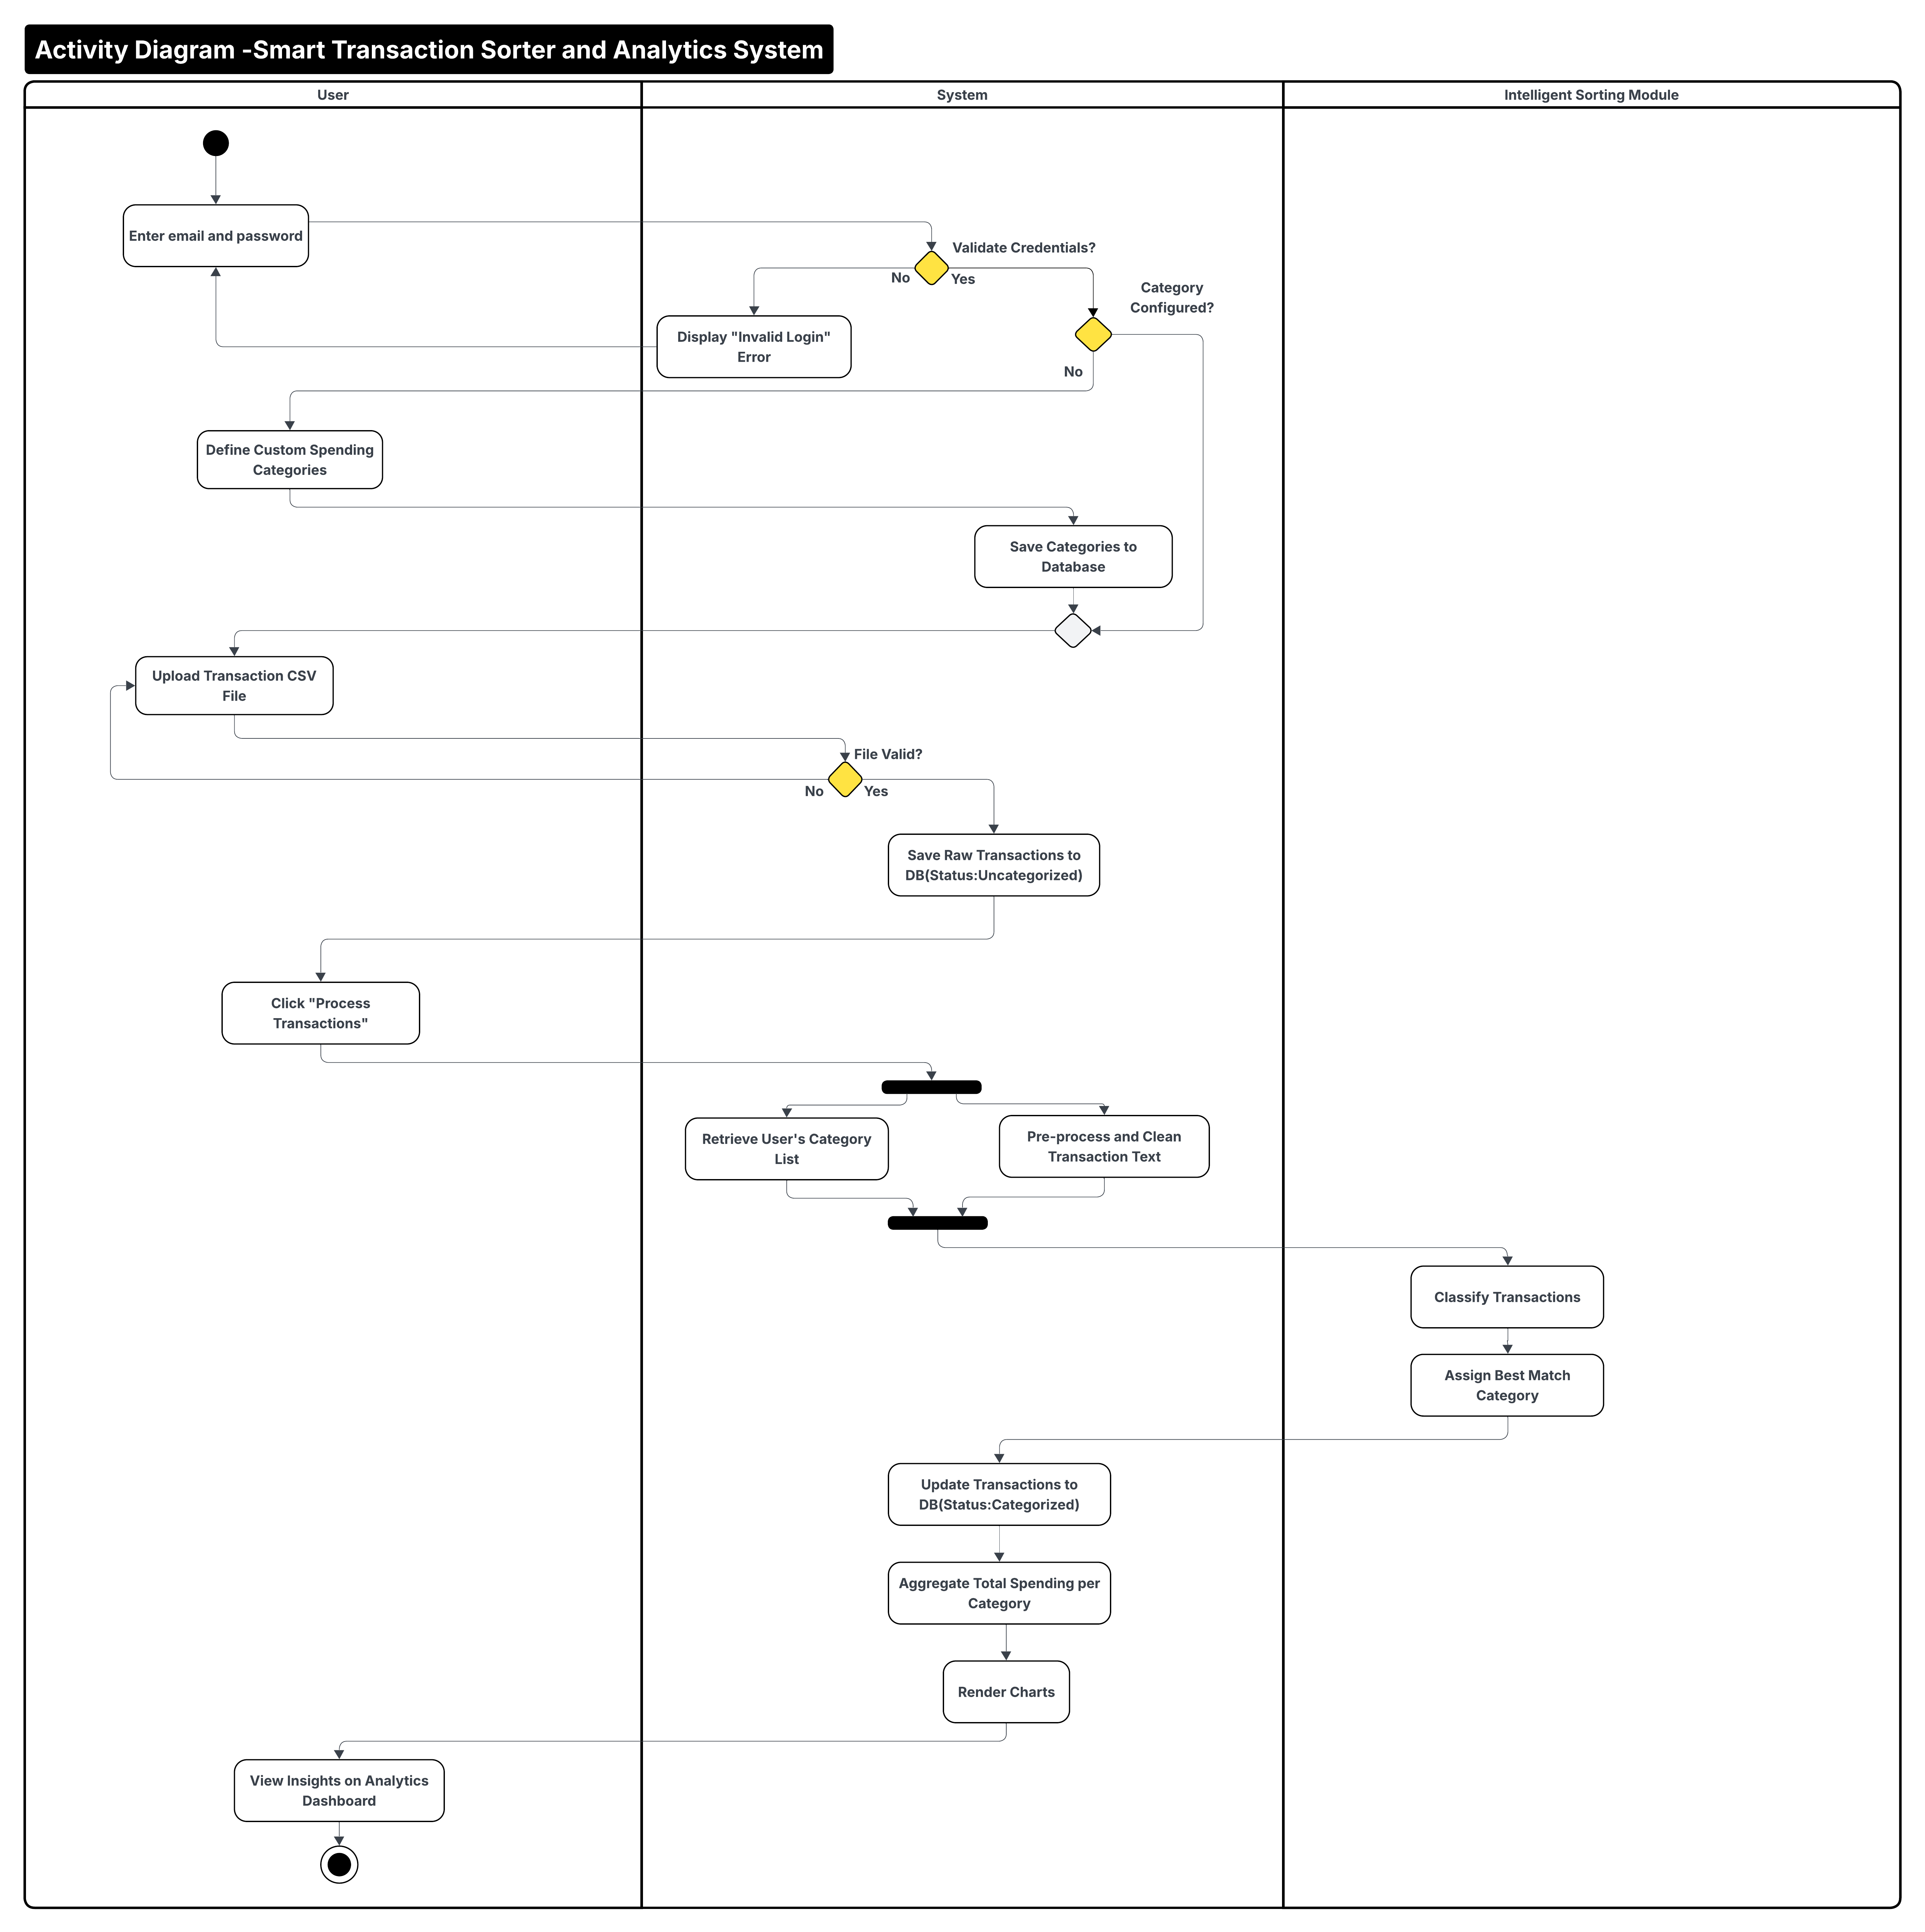
\includegraphics[height=0.85\textheight, width=1.0\textwidth, keepaspectratio]{activity_diagram.png}
		\caption{Activity Diagram: Smart Transaction Sorter and Analytics System}
		\label{fig:activity_diagram}
	\end{figure}
	
	\section{System Sequence Diagrams (SSD)}
	The System Sequence Diagram (SSD) depicts the interactions between the User, the Smart Transaction System, and the AI Engine over time. It details the specific messages exchanged during the core processes of Authentication, Data Processing, and Analytics.
	
	\begin{figure}[H]
		\centering
		% Sizing: 85% of page height to fit the long vertical flow
		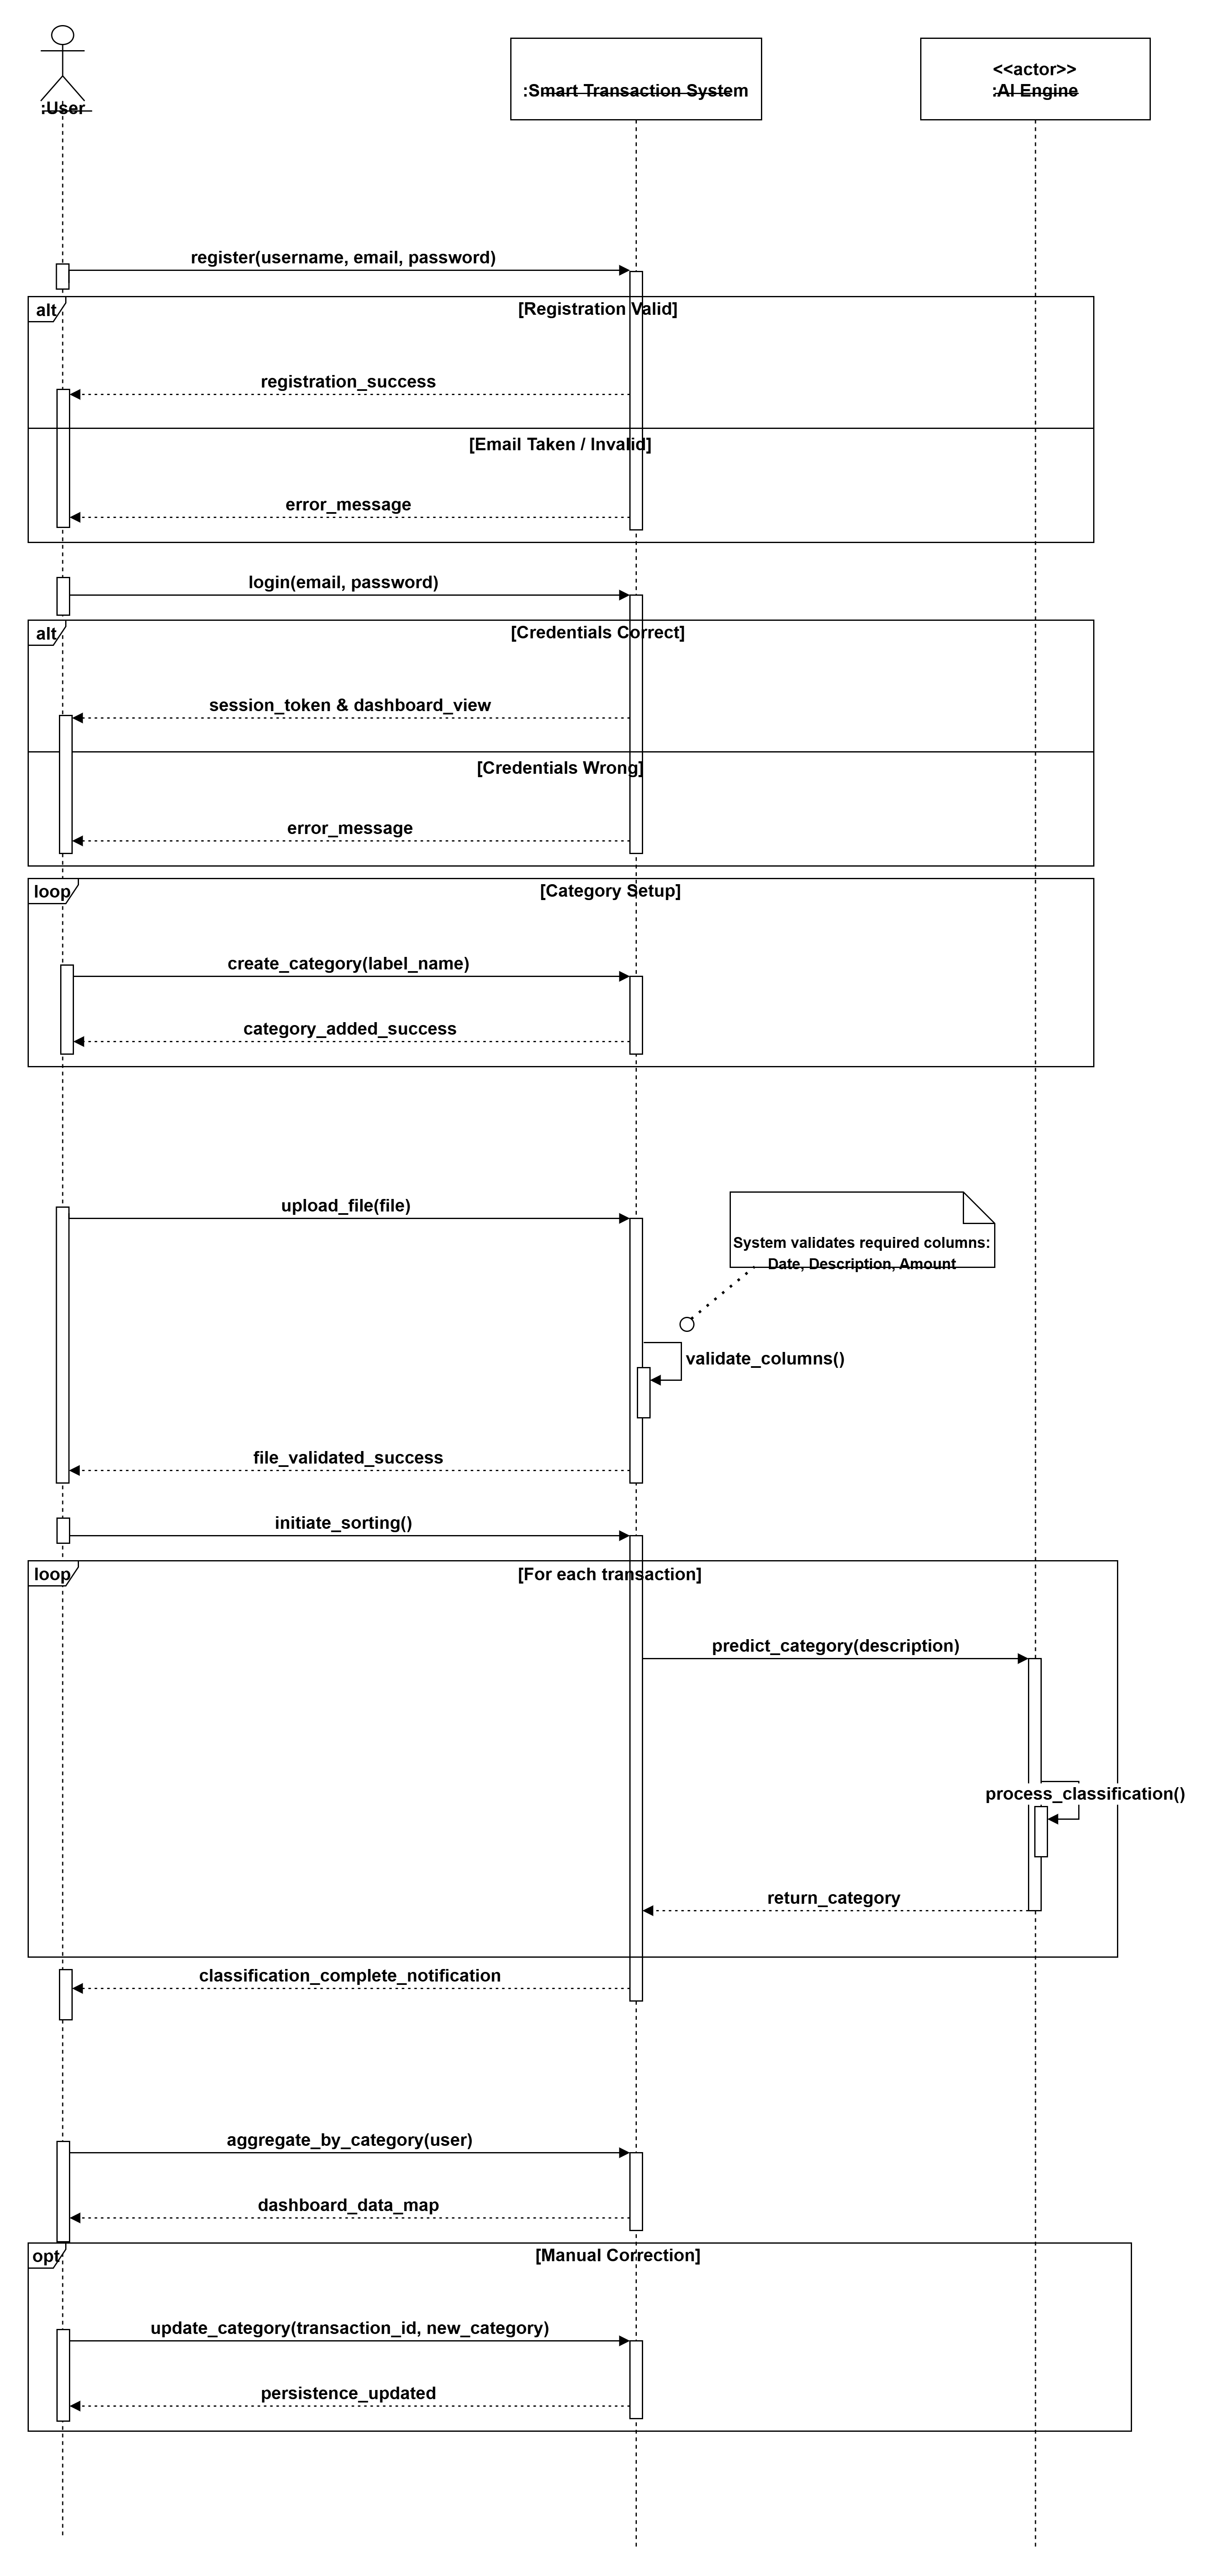
\includegraphics[height=0.85\textheight, width=1.0\textwidth, keepaspectratio]{ssd_diagram.png}
		\caption{System Sequence Diagram (SSD) for Core Workflow}
		\label{fig:ssd_diagram}
	\end{figure}
	
% =========================================================
% CHAPTER 5: SYSTEM DESIGN
% =========================================================
% =========================================================
% CHAPTER 5: SYSTEM DESIGN
% =========================================================
\chapter{System Design}

\section{Database Design}
The database design serves as the foundational data layer for the Smart Transaction Sorter. It ensures that user profiles, custom categories, and large volumes of transaction records are stored efficiently and securely. The design prioritizes data integrity and isolation between different users.

\subsection{Entity Relationship Diagram (ERD)}
The Entity Relationship Diagram (Figure \ref{fig:erd}) visualizes the logical structure of the database. It defines the entities—such as Users, Categories, and Transactions—and the relationships between them. Key relationships include the one-to-many association between a User and their Categories, ensuring that each classification schema is personalized.

\begin{figure}[H]
	\centering
	% Quotes added to handle the space in the filename safely
	\includegraphics[width=1.0\textwidth, height=0.85\textheight, keepaspectratio]{"ERD Diagram.png"}
	\caption{Entity Relationship Diagram (ERD)}
	\label{fig:erd}
\end{figure}

\section{Application Architecture}
The application architecture follows a modular structure, separating the user interface, business logic, and data handling. This separation of concerns ensures maintainability and scalability.

\subsection{Class Diagram}
The Class Diagram (Figure \ref{fig:class_diagram}) depicts the static structure of the system. It illustrates the system's classes, their attributes, methods, and the relationships between objects. This includes the Controller classes that handle logic, Service classes that manage data processing, and Model classes that represent the database entities.

\begin{figure}[H]
	\centering
	% Quotes added to handle the space in the filename safely
	\includegraphics[width=1.0\textwidth, height=0.90\textheight, keepaspectratio]{"Class Diagram.png"}
	\caption{System Class Diagram}
	\label{fig:class_diagram}
\end{figure}

\subsection{Interaction Design (Sequence Diagrams)}
This section details the dynamic behavior of the system. The following Sequence Diagrams illustrate the step-by-step message flow between system objects for the most critical use cases, from the initial user action to the final system response.

% --- 1. Registration ---
\subsubsection{User Registration Workflow}
This interaction details the process of creating a new user account, including validation of unique email addresses and secure password hashing before storage.
\begin{figure}[H]
	\centering
	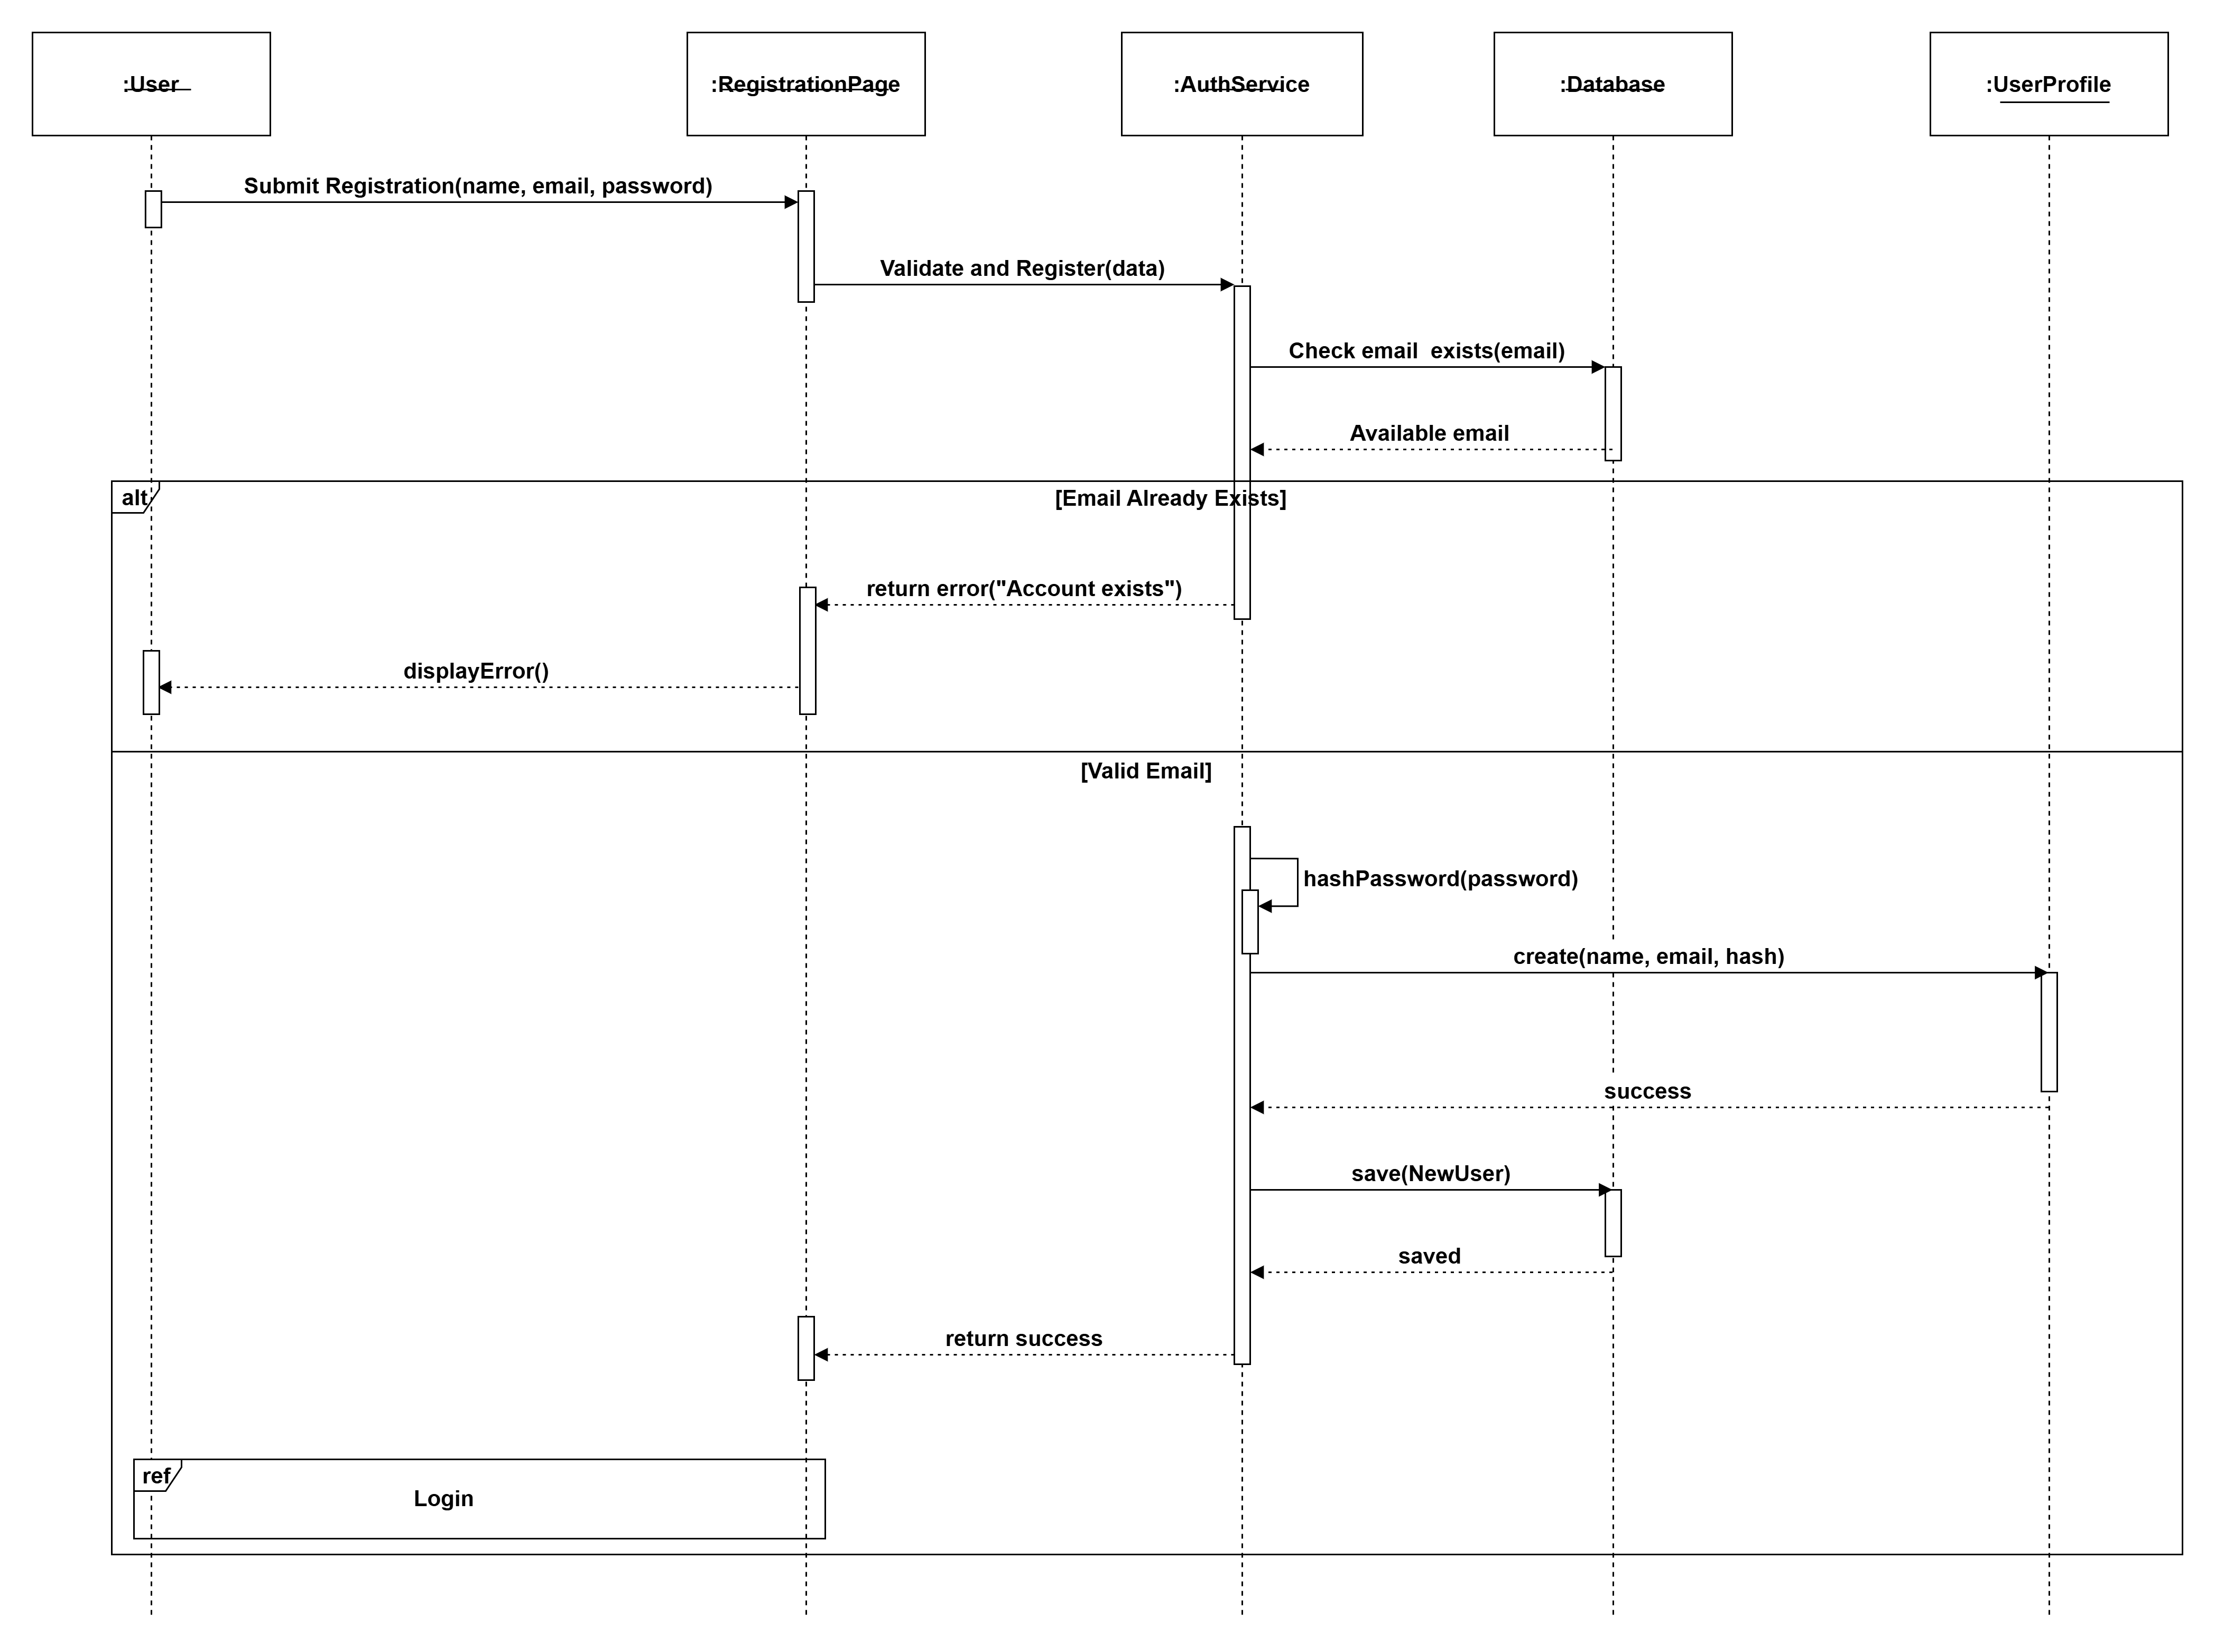
\includegraphics[width=1.0\textwidth, height=0.85\textheight, keepaspectratio]{seq_register.png}
	\caption{Sequence Diagram: User Registration}
	\label{fig:seq_register}
\end{figure}

% --- 2. Login ---
\subsubsection{Secure Login Workflow}
This diagram illustrates the authentication process, verifying credentials against the database and generating a session token upon success.
\begin{figure}[H]
	\centering
	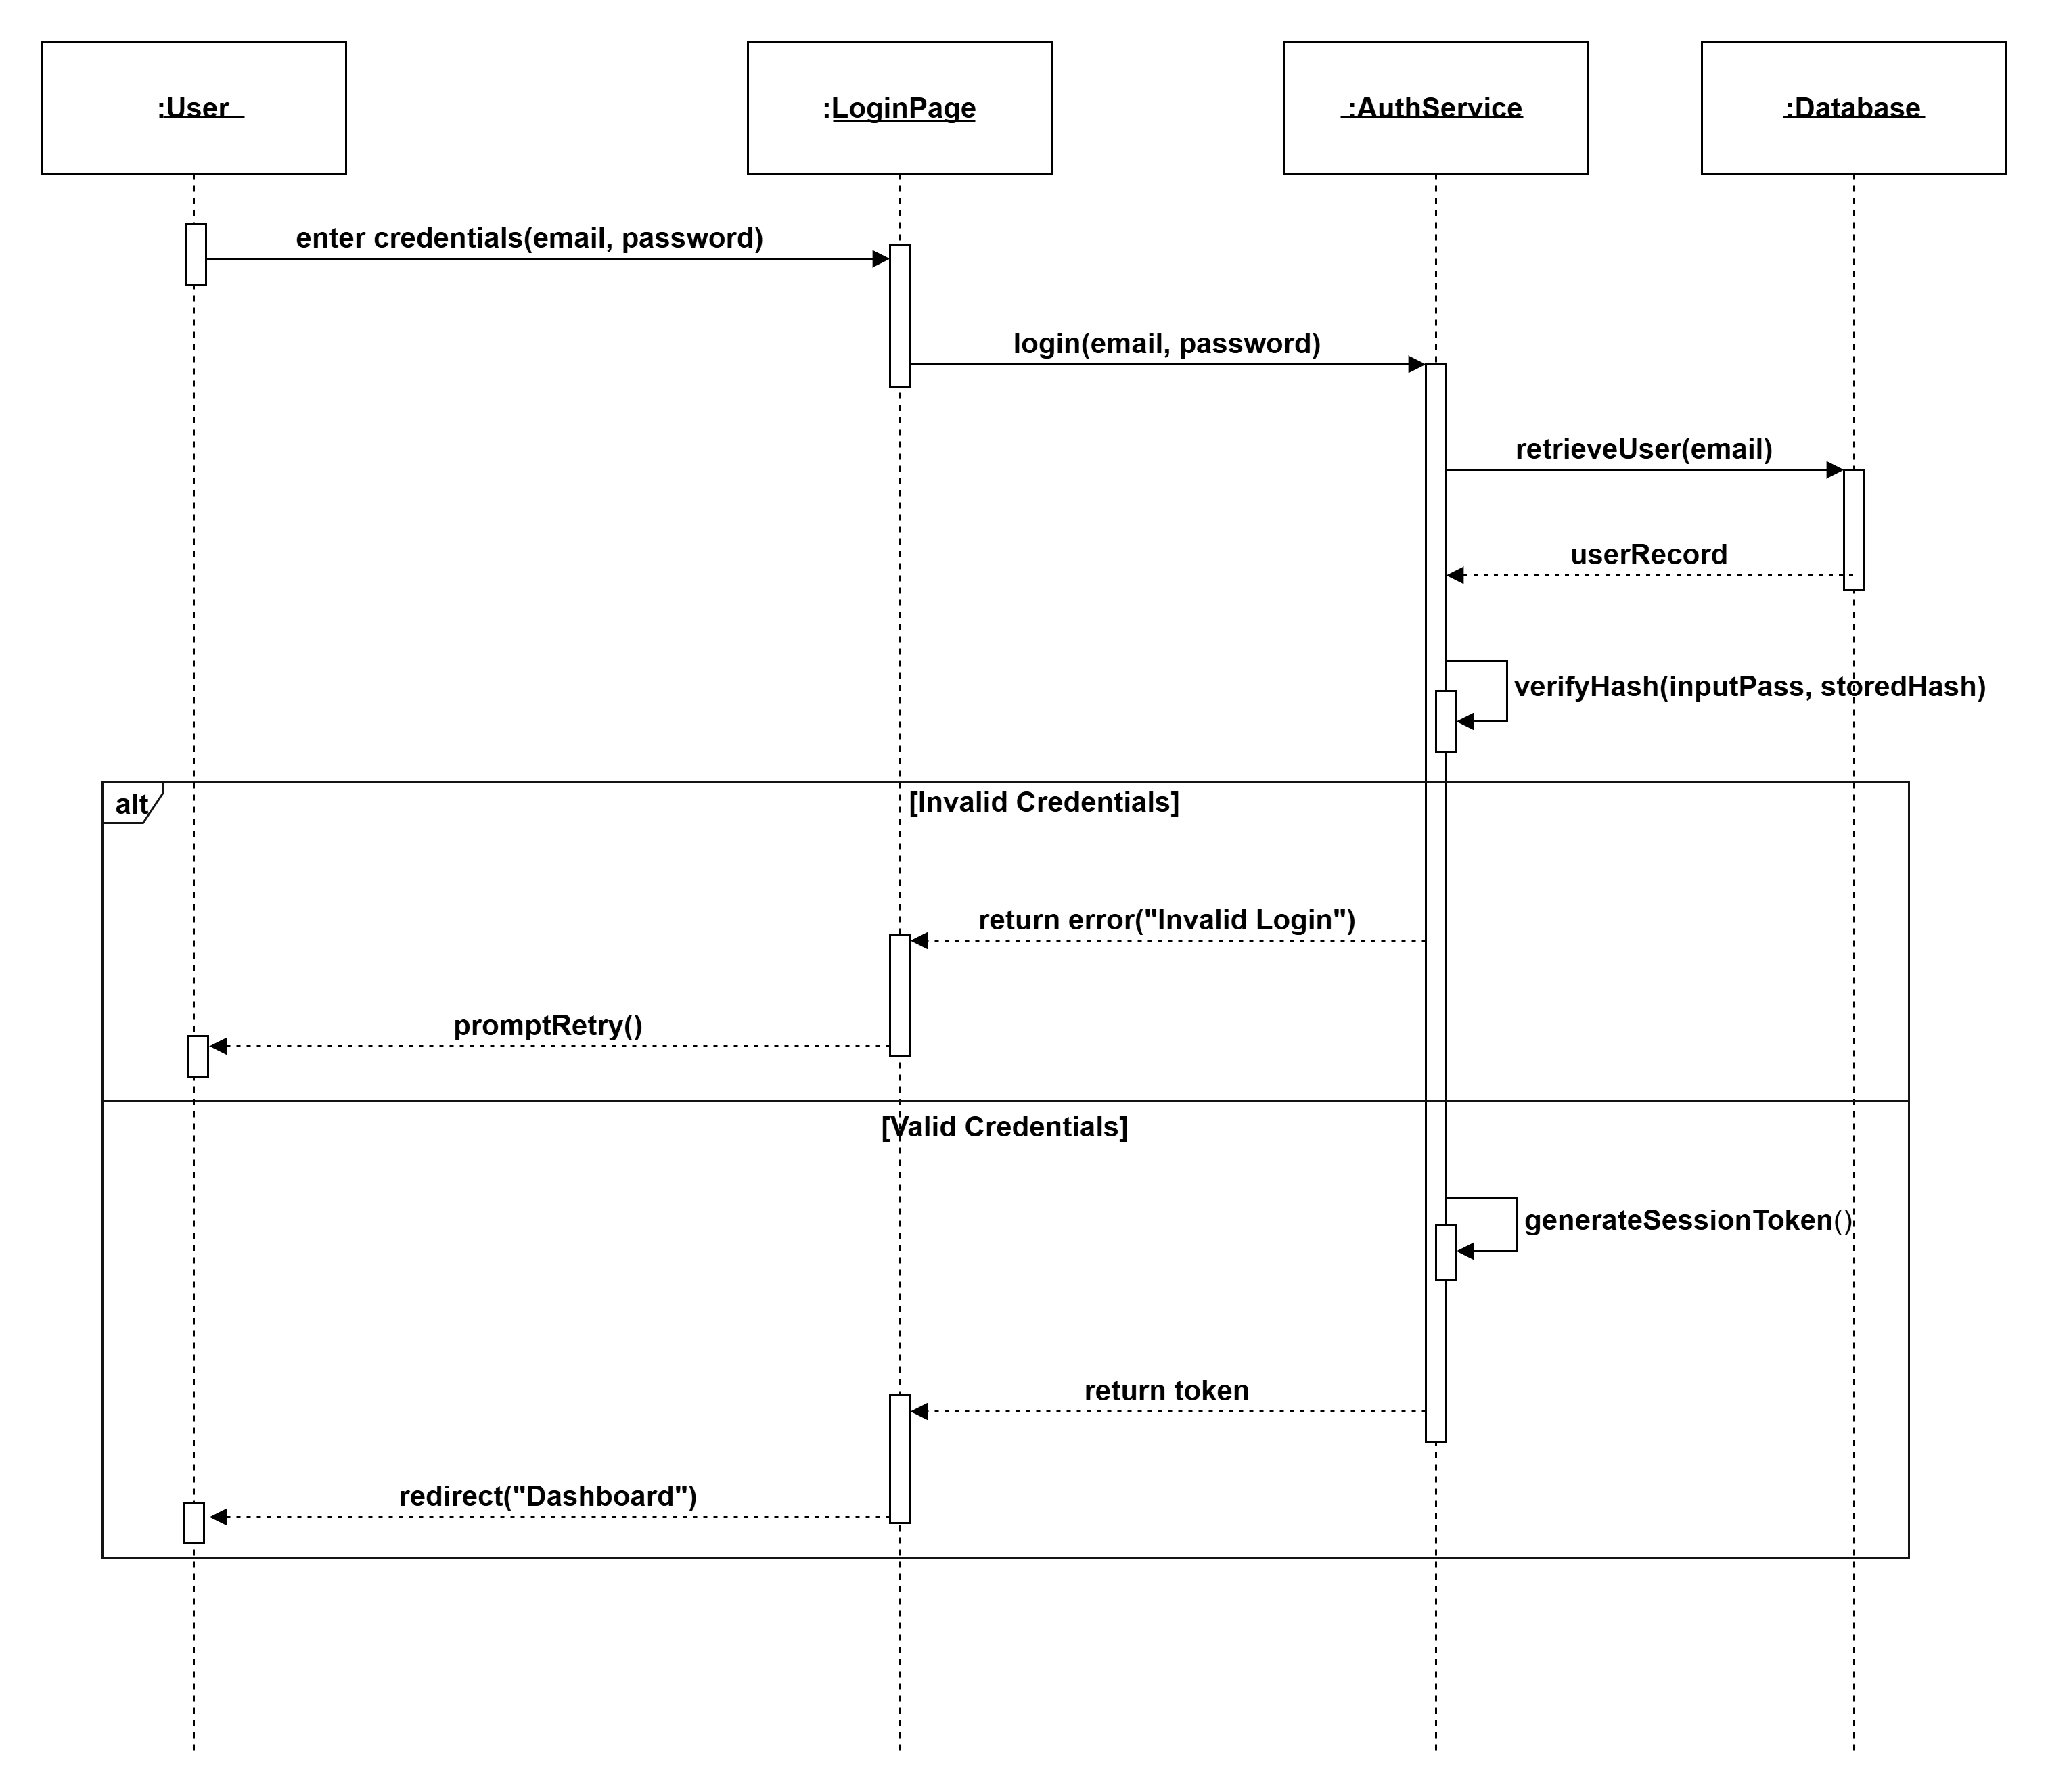
\includegraphics[width=1.0\textwidth, height=0.85\textheight, keepaspectratio]{seq_login.png}
	\caption{Sequence Diagram: User Login}
	\label{fig:seq_login}
\end{figure}

% --- 3. Categories ---
\subsubsection{Manage Spending Categories Workflow}
This flow demonstrates how a user defines custom spending labels (e.g., "Gym", "Groceries") and how the system prevents duplicate category entries.
\begin{figure}[H]
	\centering
	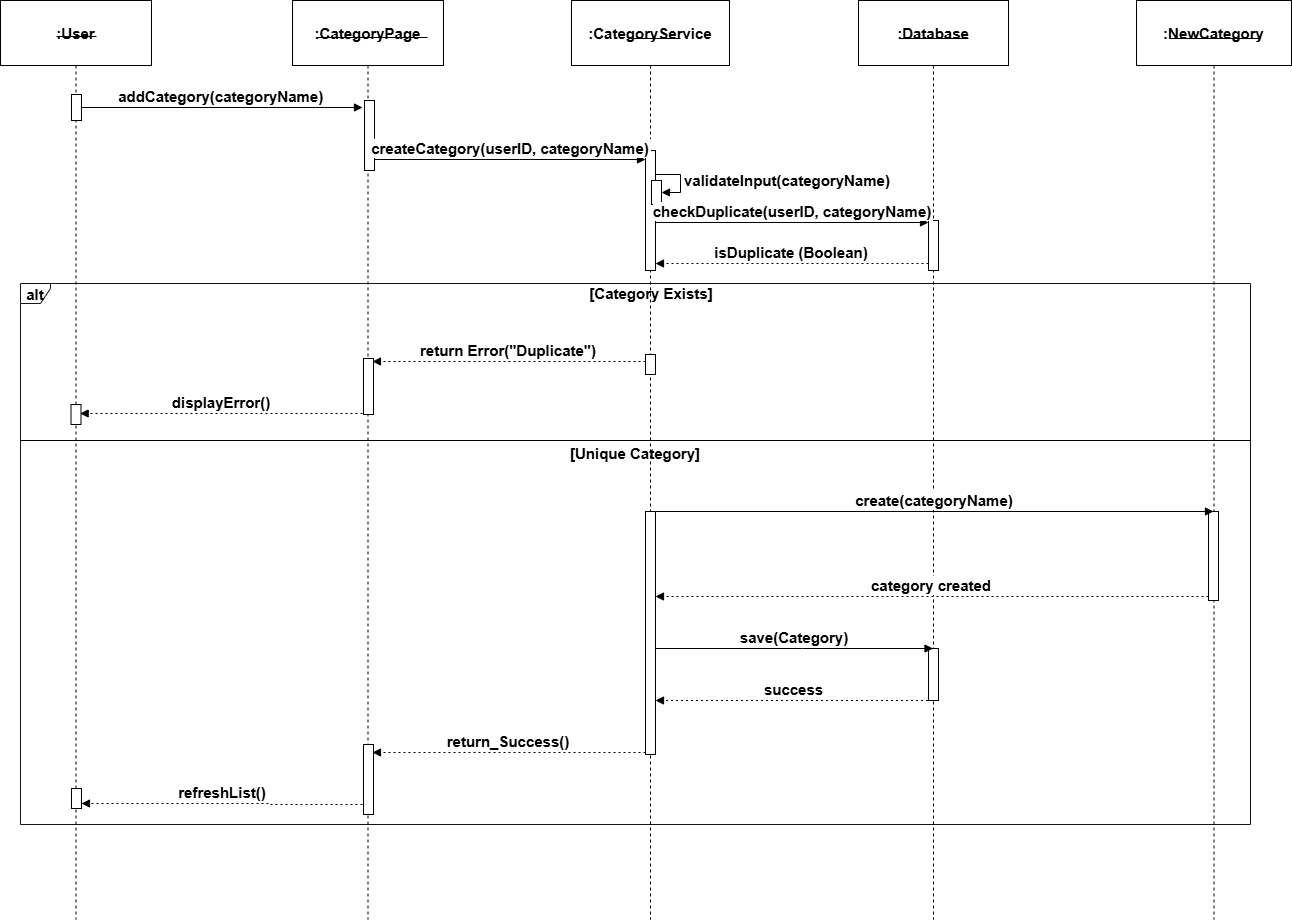
\includegraphics[width=1.0\textwidth, height=0.85\textheight, keepaspectratio]{seq_categories.png}
	\caption{Sequence Diagram: Manage Custom Categories}
	\label{fig:seq_categories}
\end{figure}

% --- 4. Upload ---
\subsubsection{CSV Data Upload Workflow}
This diagram covers the data ingestion process, including file extension validation (.csv), structure verification (checking columns), and saving raw data.
\begin{figure}[H]
	\centering
	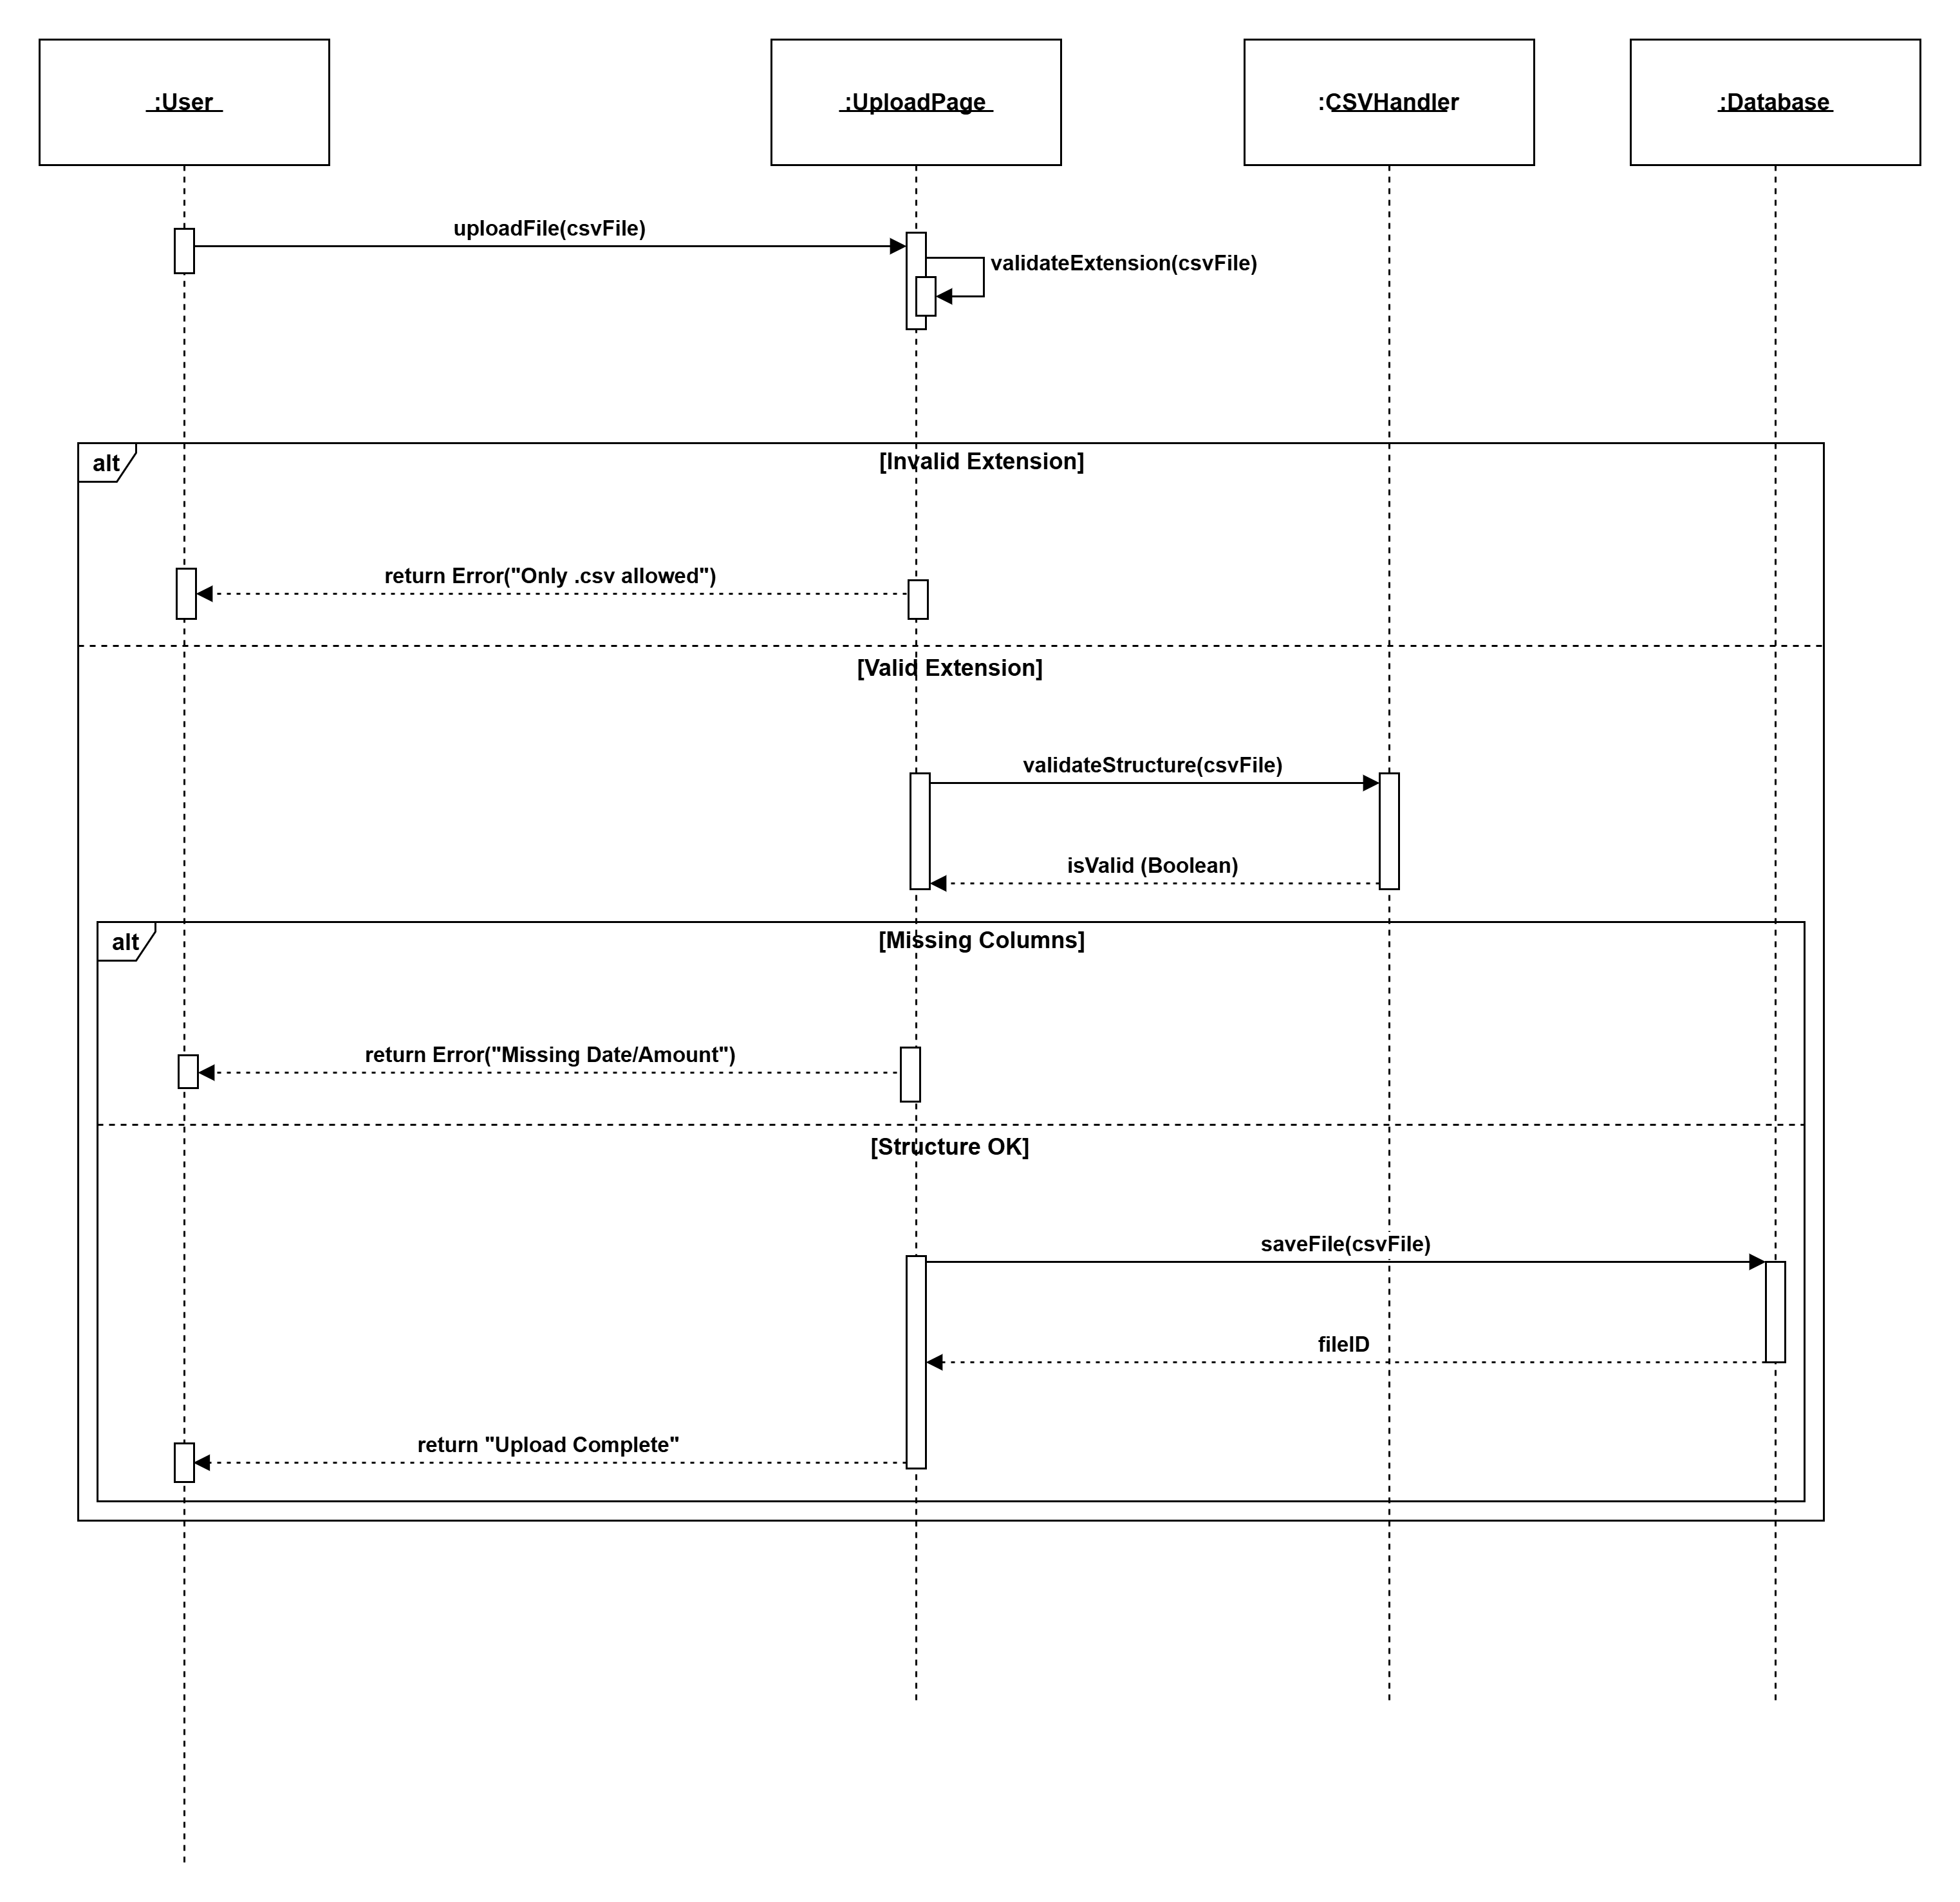
\includegraphics[width=1.0\textwidth, height=0.85\textheight, keepaspectratio]{seq_upload.png}
	\caption{Sequence Diagram: CSV Data Upload}
	\label{fig:seq_upload}
\end{figure}

% --- 5. AI Processing ---
\subsubsection{AI Transaction Processing Workflow}
This is the core system process. It depicts the loop where the AI Engine reads each transaction, predicts the best category based on the user's list, and updates the record.
\begin{figure}[H]
	\centering
	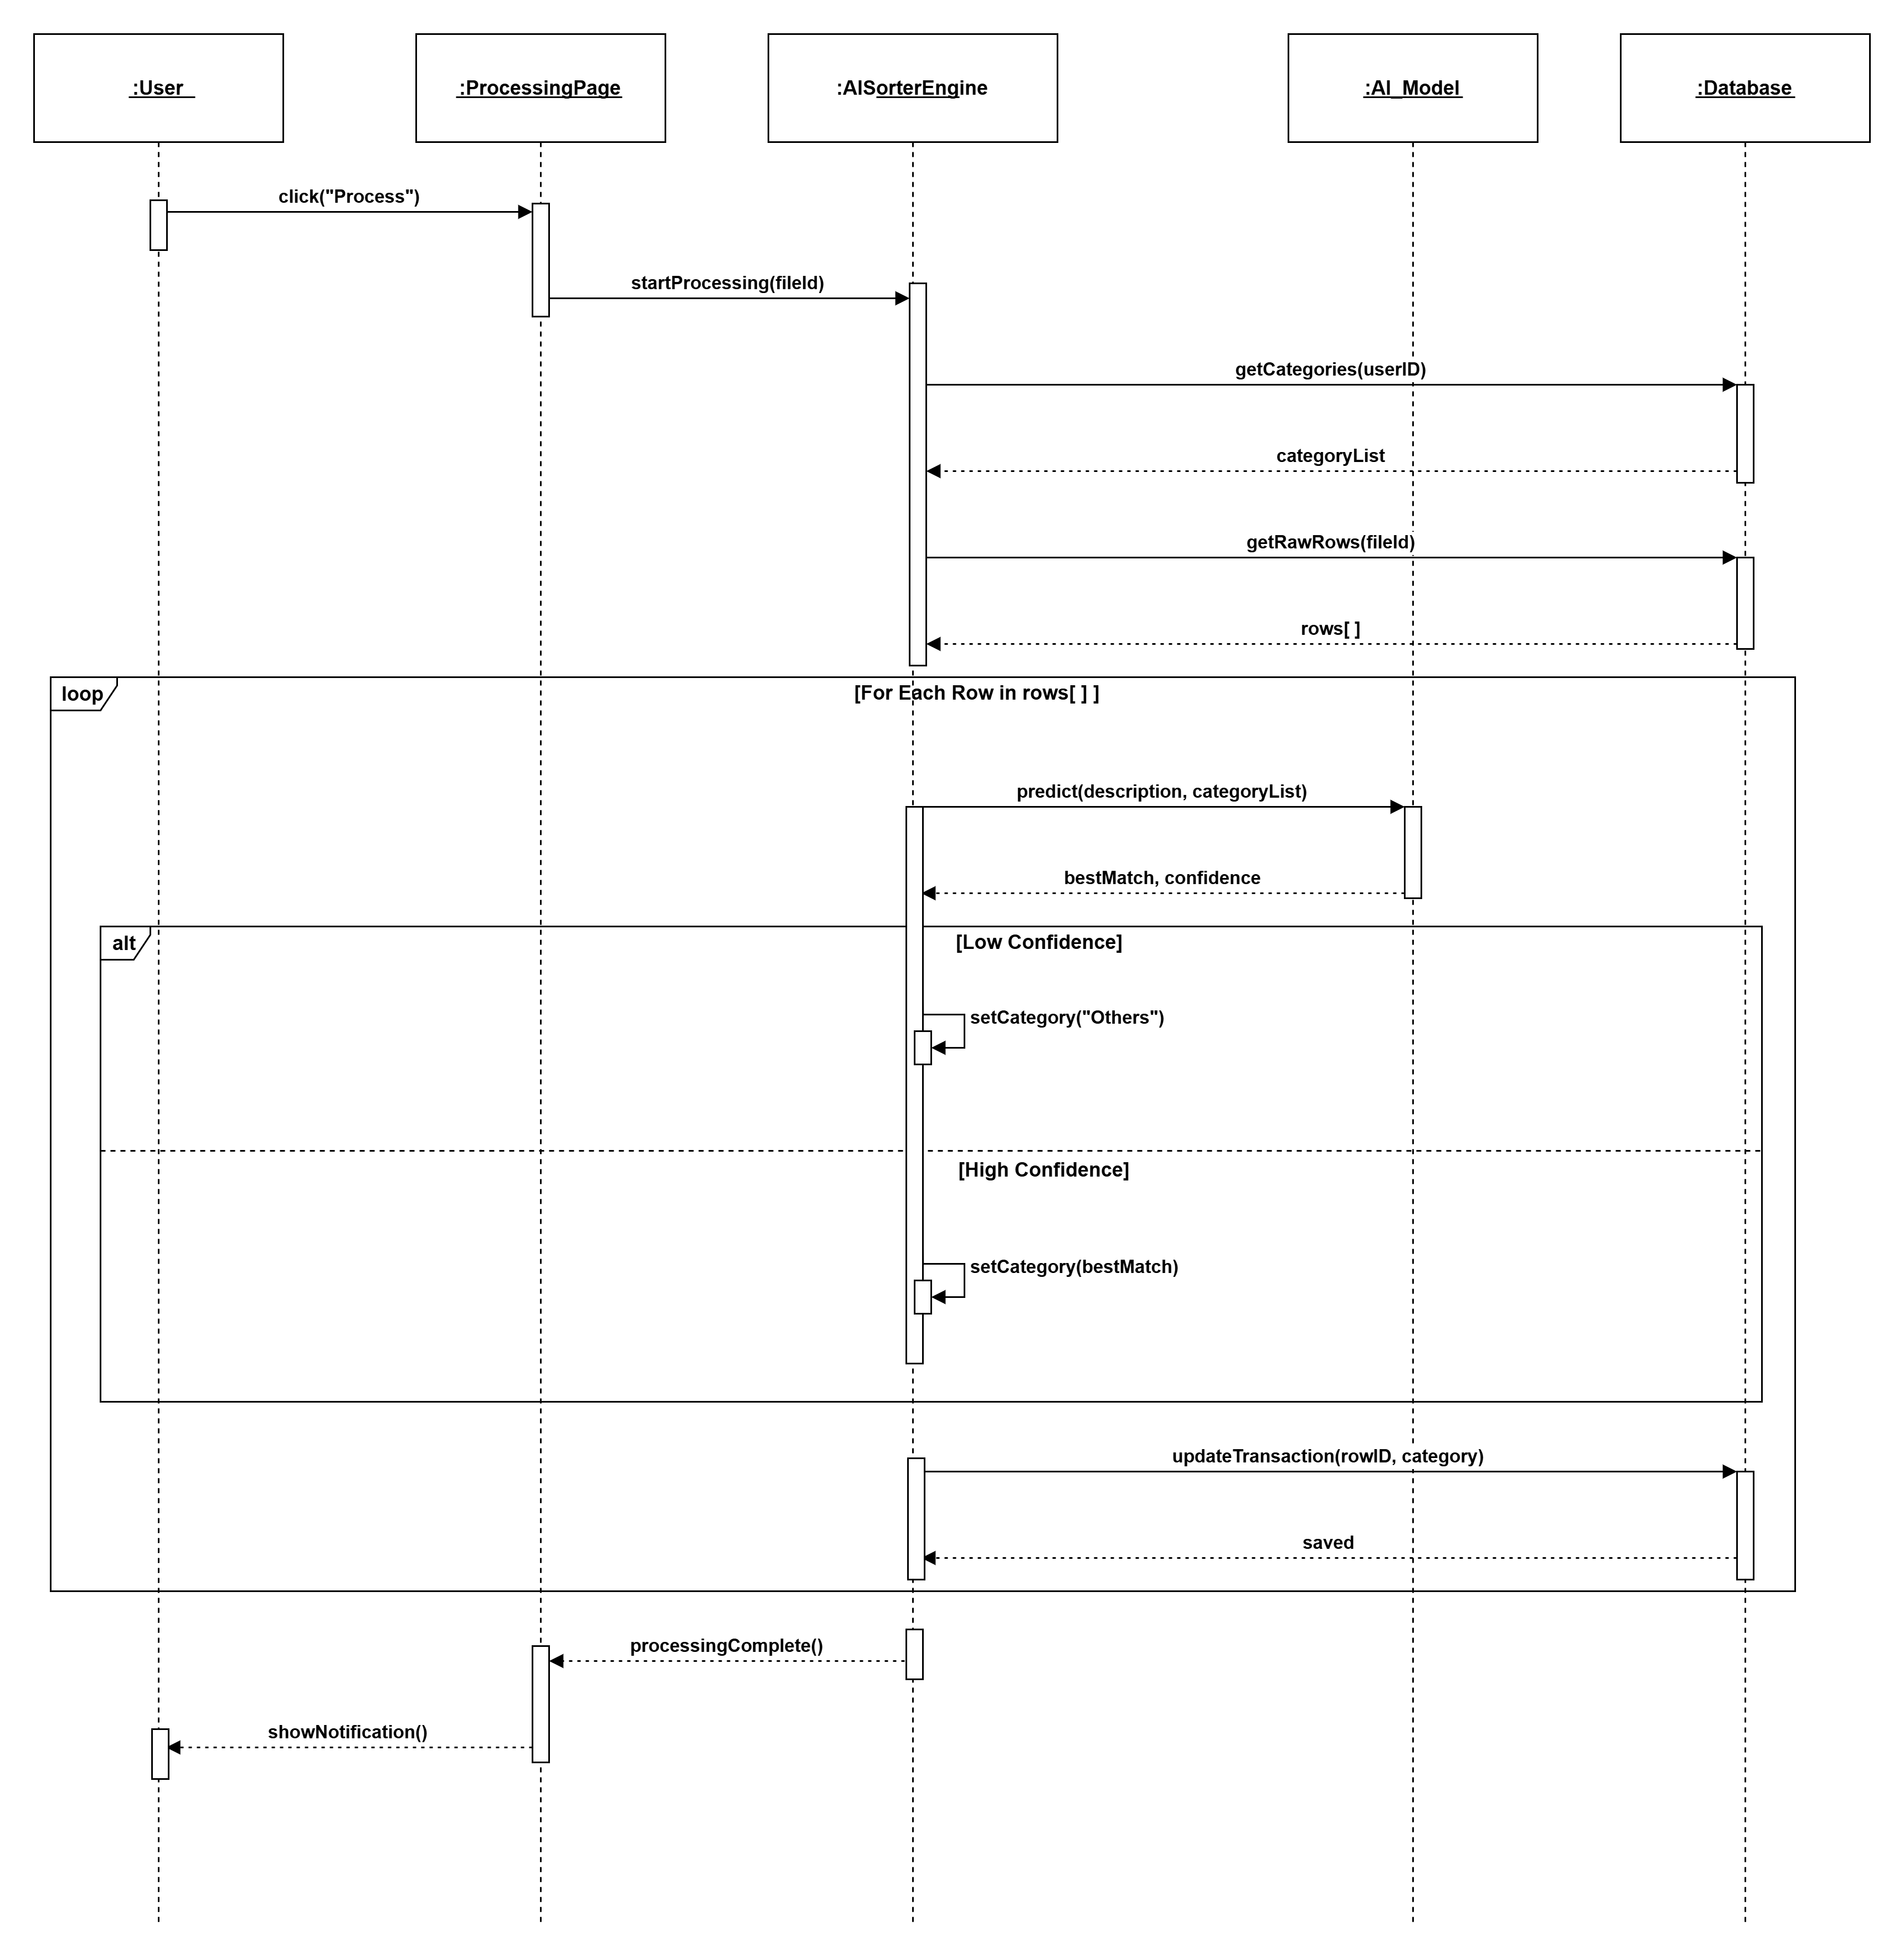
\includegraphics[width=1.0\textwidth, height=0.85\textheight, keepaspectratio]{seq_ai_process.png}
	\caption{Sequence Diagram: AI Transaction Processing}
	\label{fig:seq_ai}
\end{figure}

% --- 6. Dashboard ---
\subsubsection{Dashboard Analytics Workflow}
This interaction shows how the system aggregates classified data from the database and delivers the JSON structure required to render the frontend charts.
\begin{figure}[H]
	\centering
	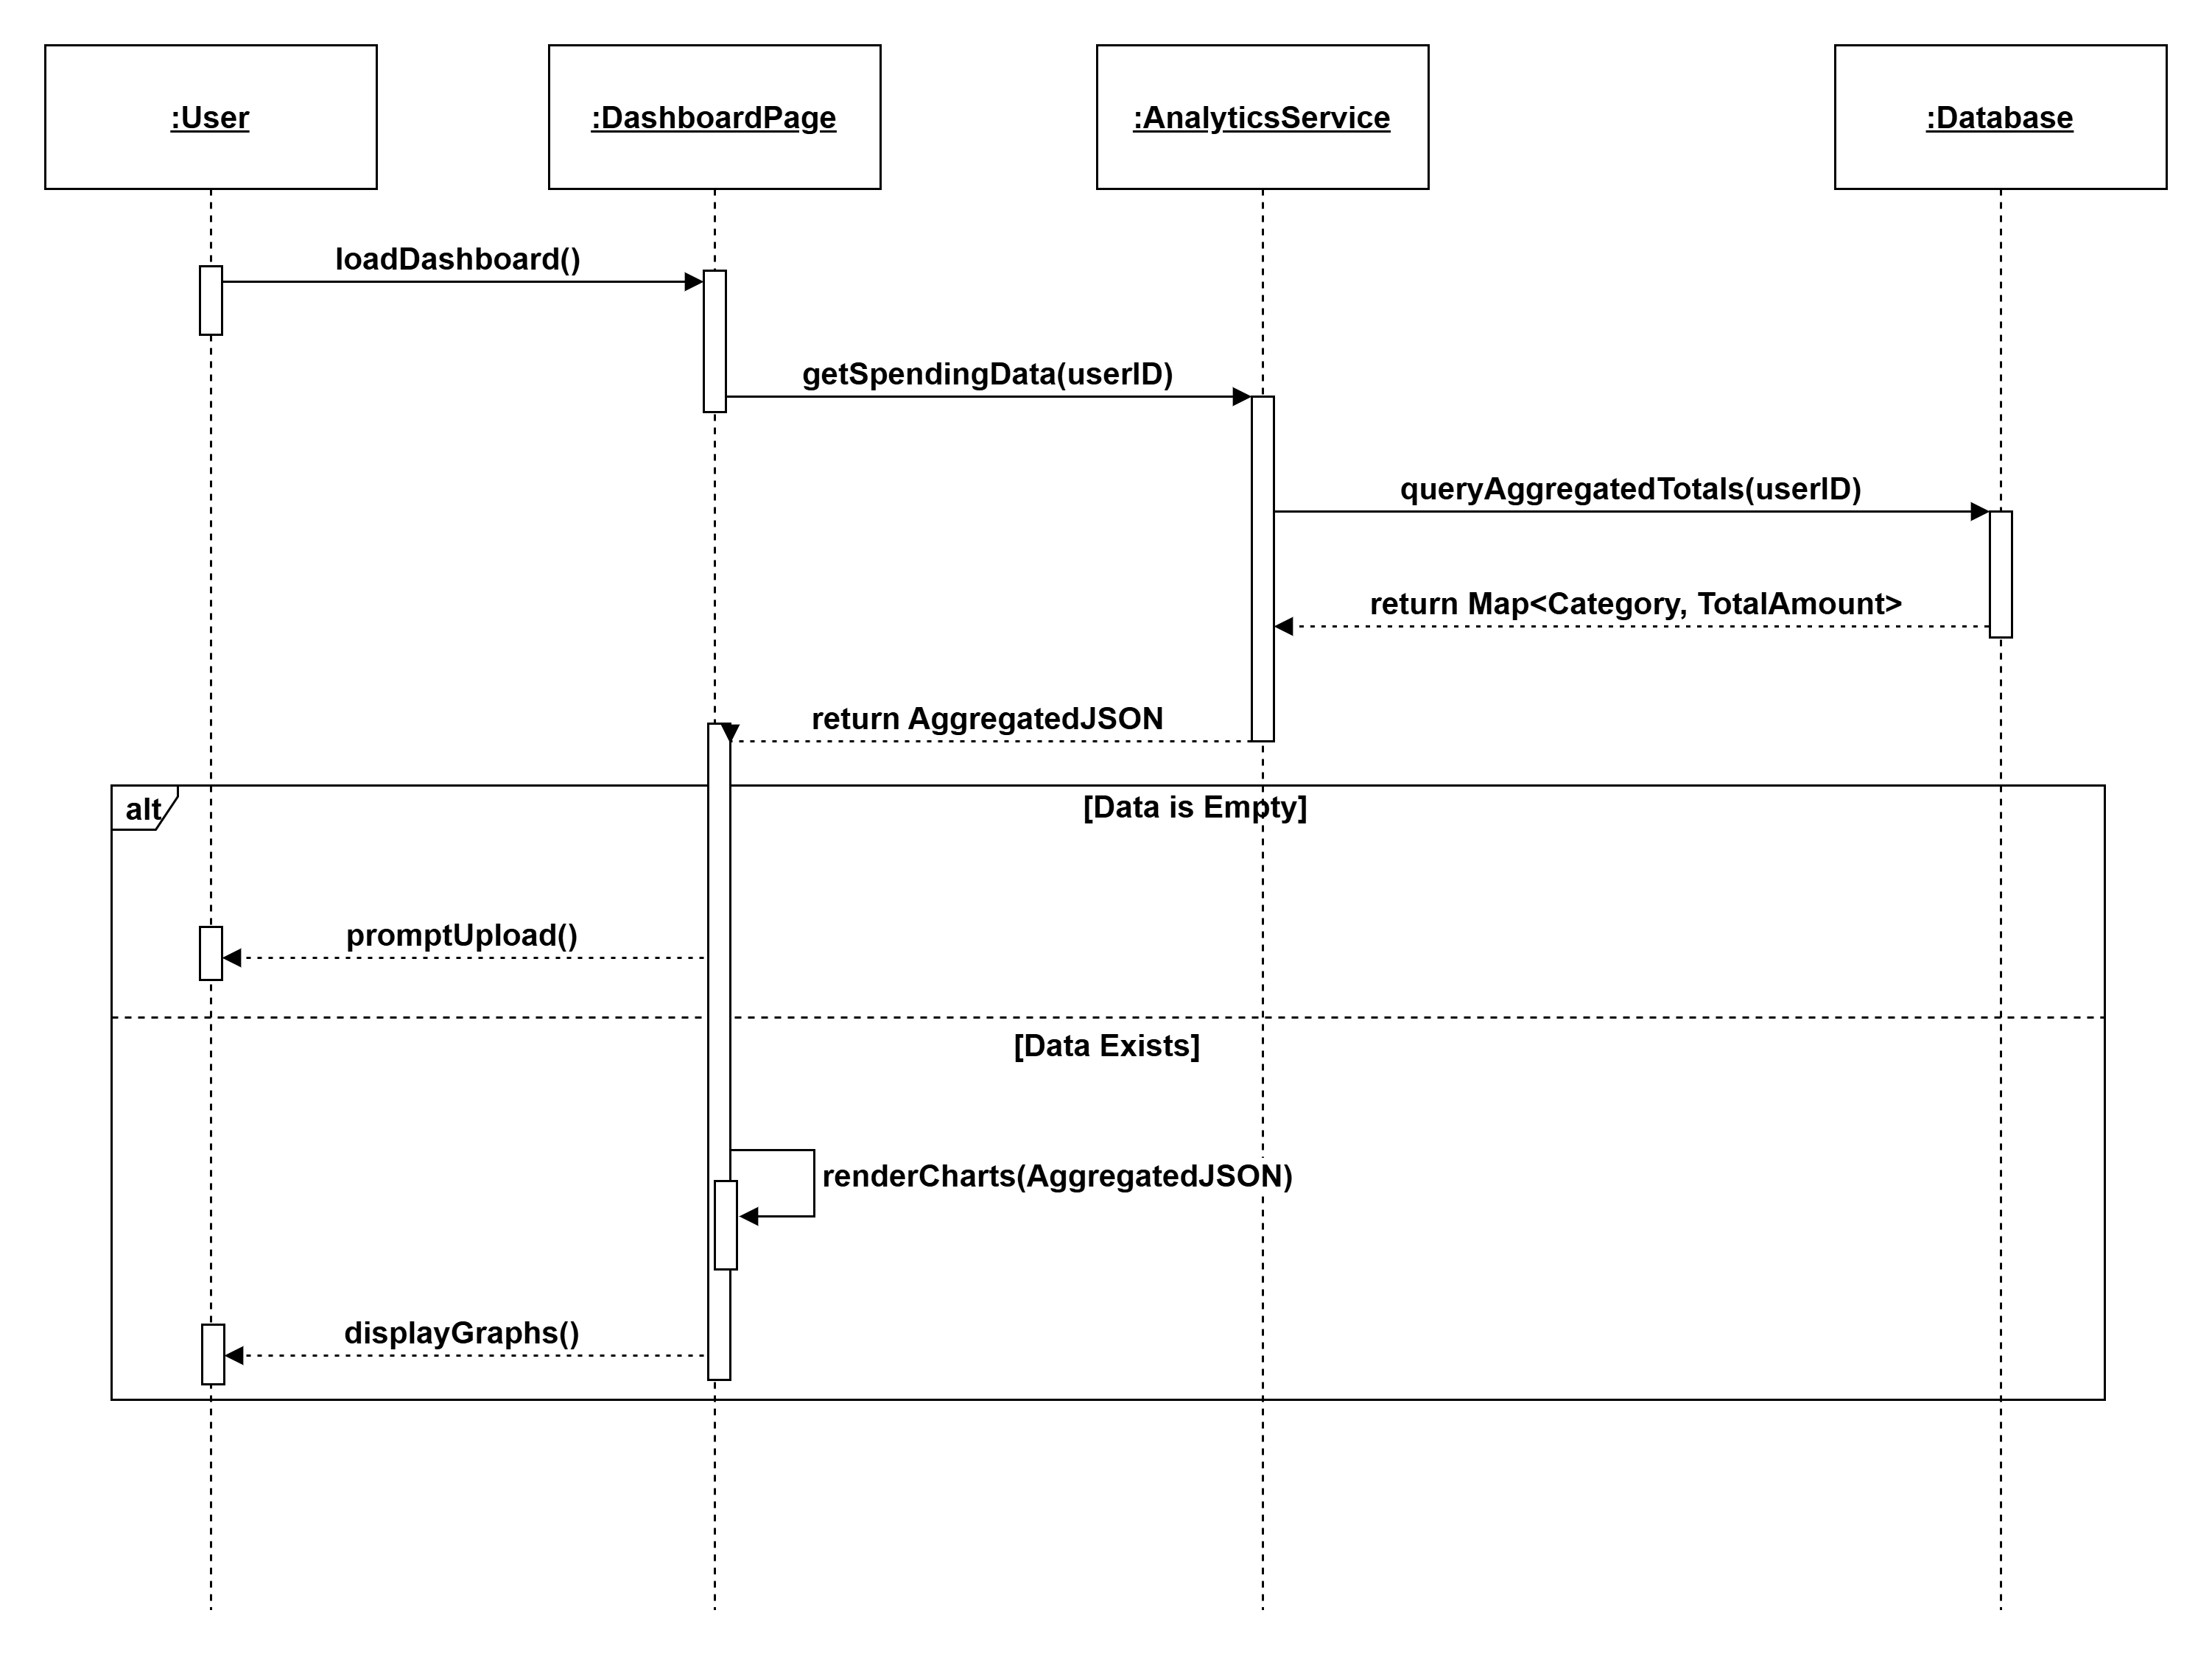
\includegraphics[width=1.0\textwidth, height=0.85\textheight, keepaspectratio]{seq_dashboard.png}
	\caption{Sequence Diagram: Dashboard Analytics}
	\label{fig:seq_dashboard}
\end{figure}

% --- 7. Delete ---
\subsubsection{Data Deletion Workflow}
This diagram illustrates the privacy feature allowing users to permanently erase their data, including the confirmation popup logic to prevent accidental deletion.
\begin{figure}[H]
	\centering
	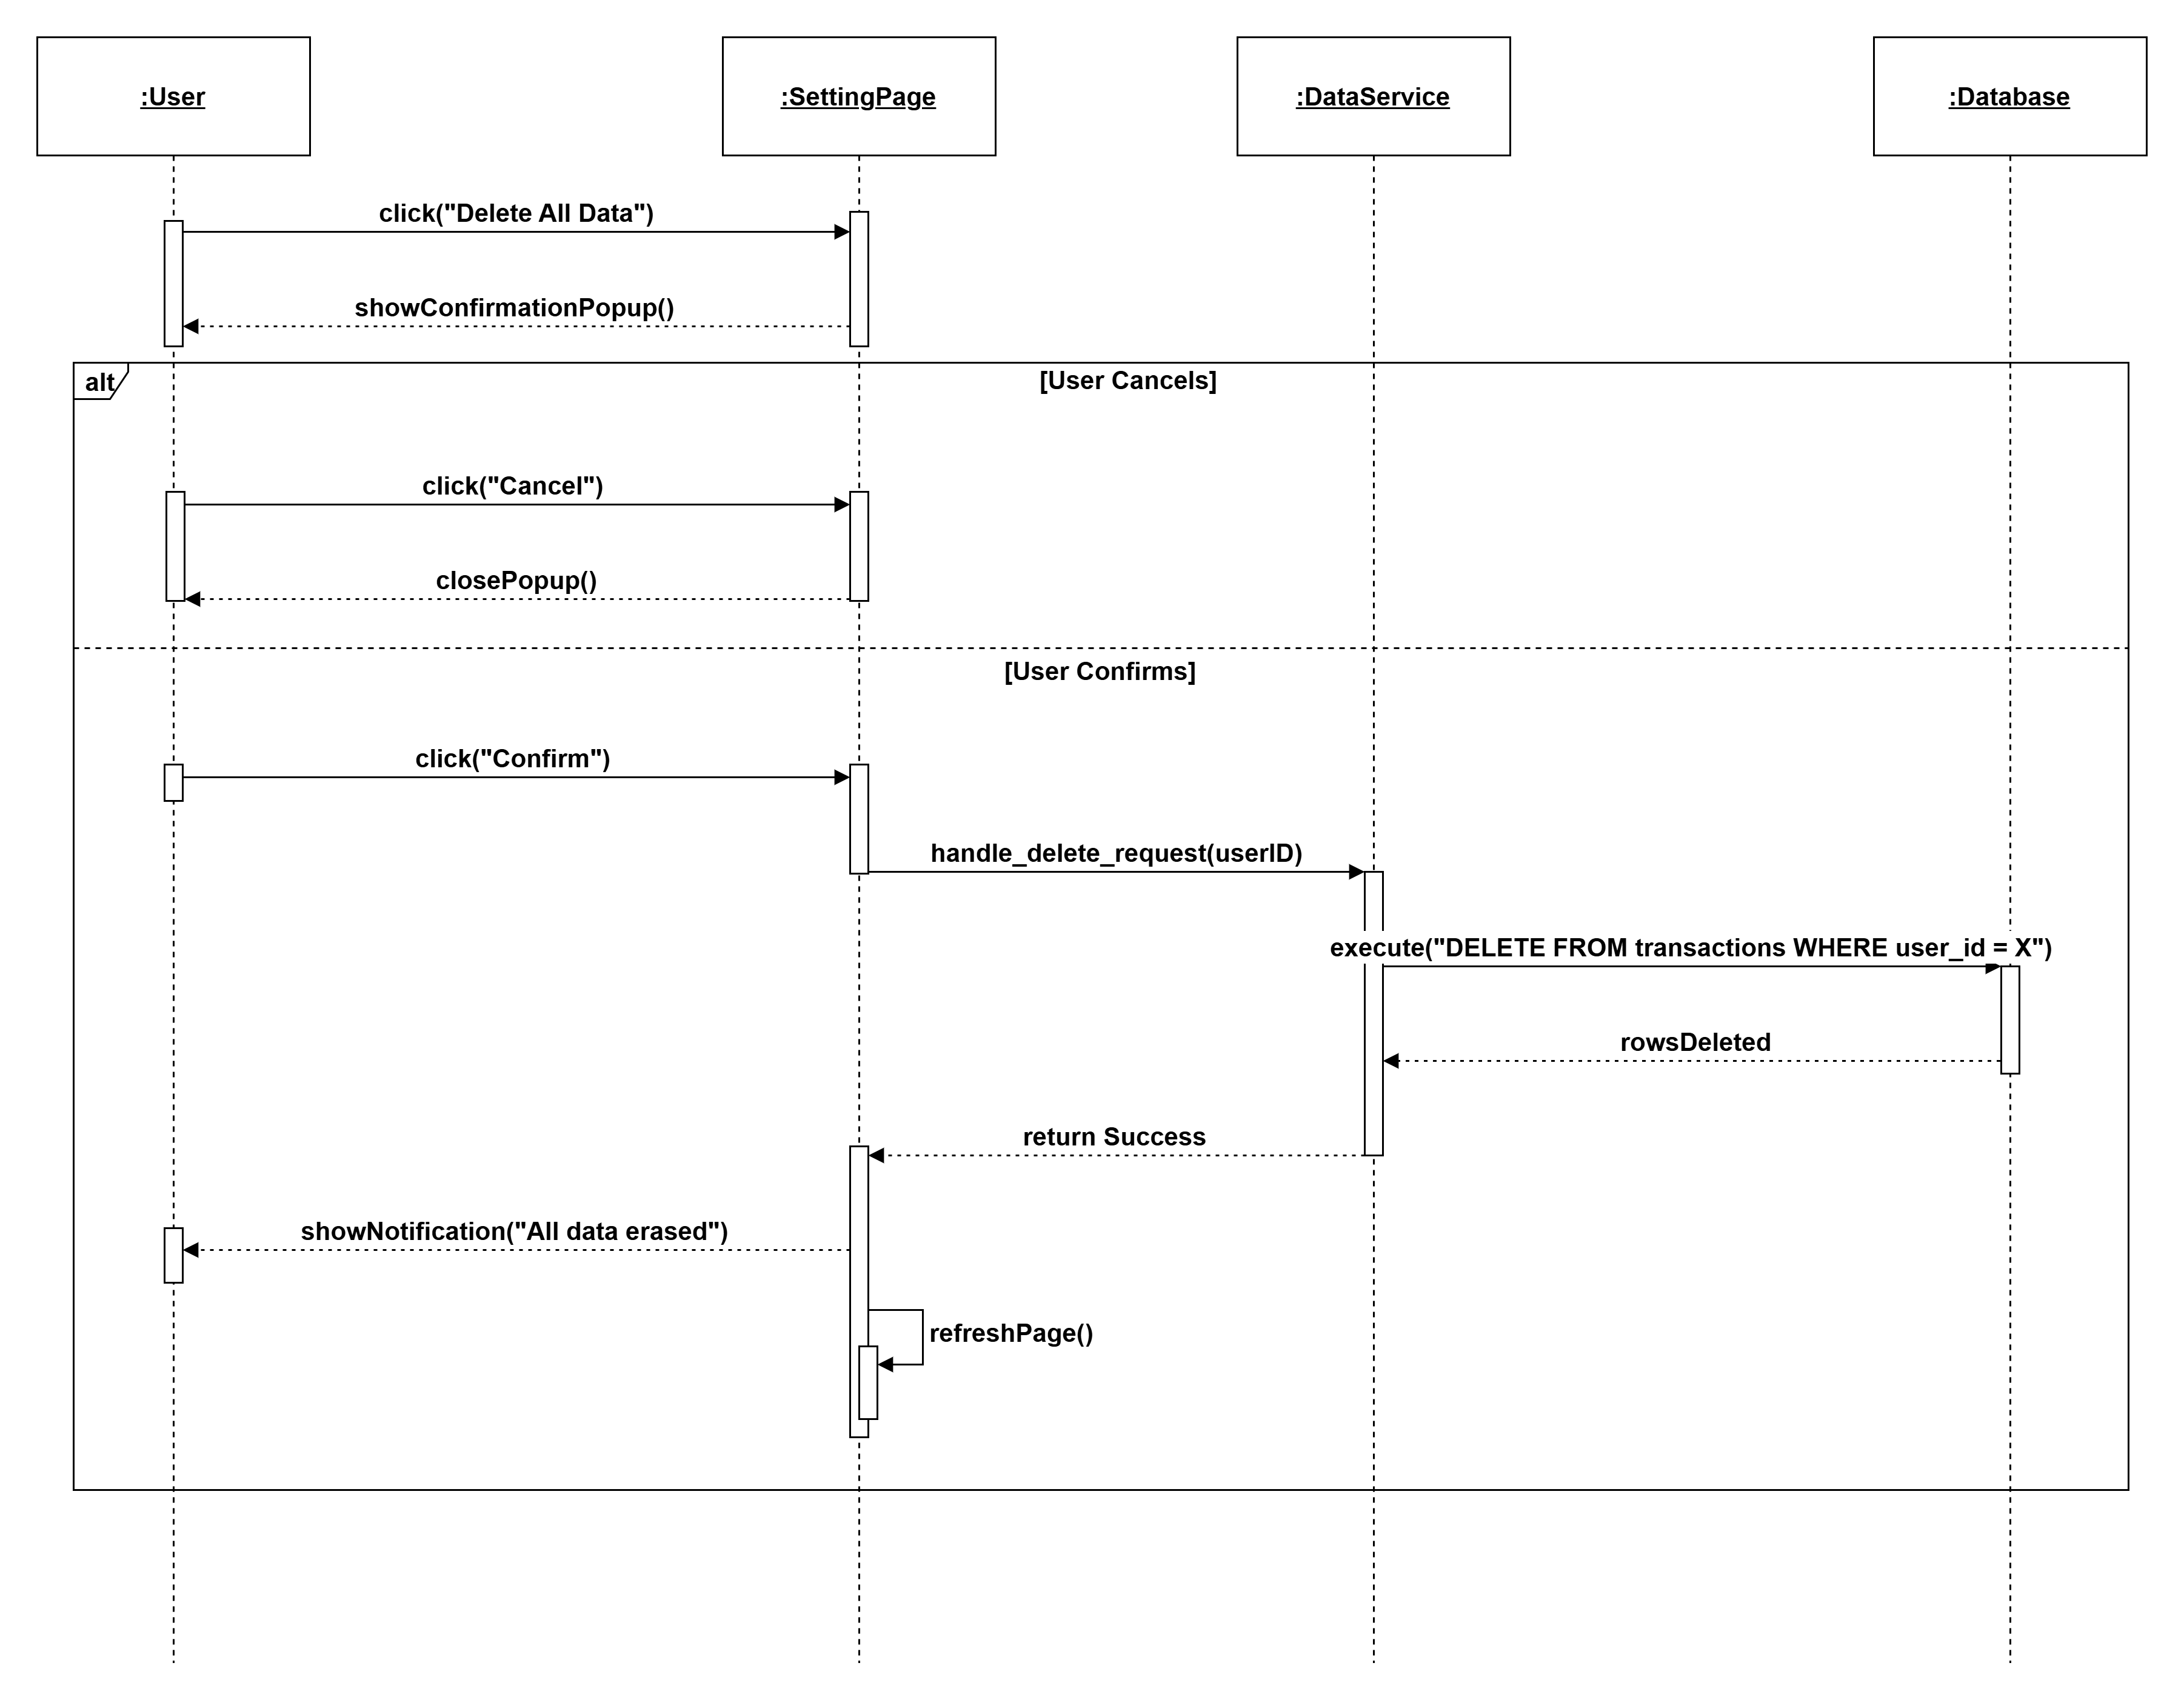
\includegraphics[width=1.0\textwidth, height=0.85\textheight, keepaspectratio]{seq_delete.png}
	\caption{Sequence Diagram: Delete All User Data}
	\label{fig:seq_delete}
\end{figure}

% --- 8. Admin ---
\subsubsection{Admin User Management Workflow}
This final diagram details the administrative capabilities, such as searching for specific users in the system and performing account management actions.
\begin{figure}[H]
	\centering
	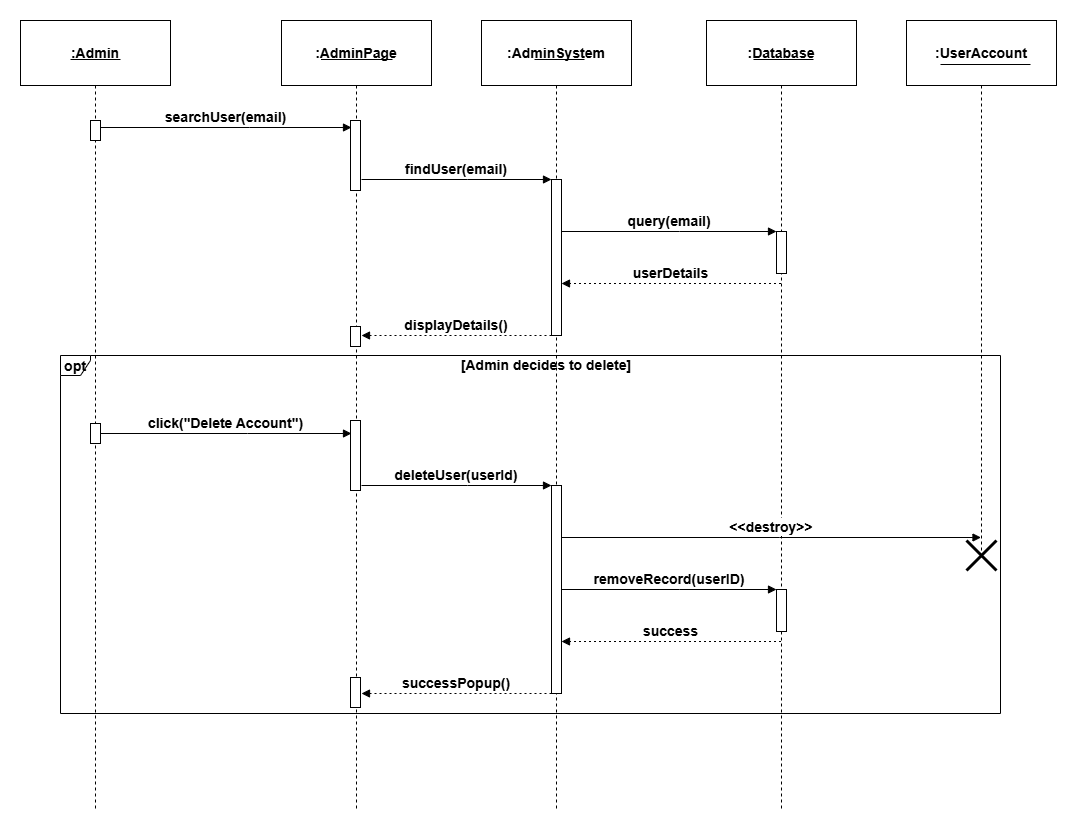
\includegraphics[width=1.0\textwidth, height=0.85\textheight, keepaspectratio]{seq_admin.png}
	\caption{Sequence Diagram: Admin User Management}
	\label{fig:seq_admin}
\end{figure}

\section{Physical Architecture (Deployment)}
The Physical Architecture describes the hardware and software environment in which the system runs. It outlines the deployment nodes, including the client devices (browsers), the web server hosting the Django application, and the database server. The specific configurations are detailed below:

\begin{itemize}
	\item \textbf{Client Node:} Represents the end-user's device (Laptop/Mobile) running a modern web browser (e.g., Chrome, Edge) to access the application via HTTPS.
	\item \textbf{Application Server Node:} The central processing unit hosting the Django web server and the AI Classification Engine. It handles HTTP requests and business logic.
	\item \textbf{Database Node:} A dedicated storage server (PostgreSQL) responsible for persistent data storage, secure transaction logging, and query retrieval.
\end{itemize}

\begin{figure}[H]
	\centering
	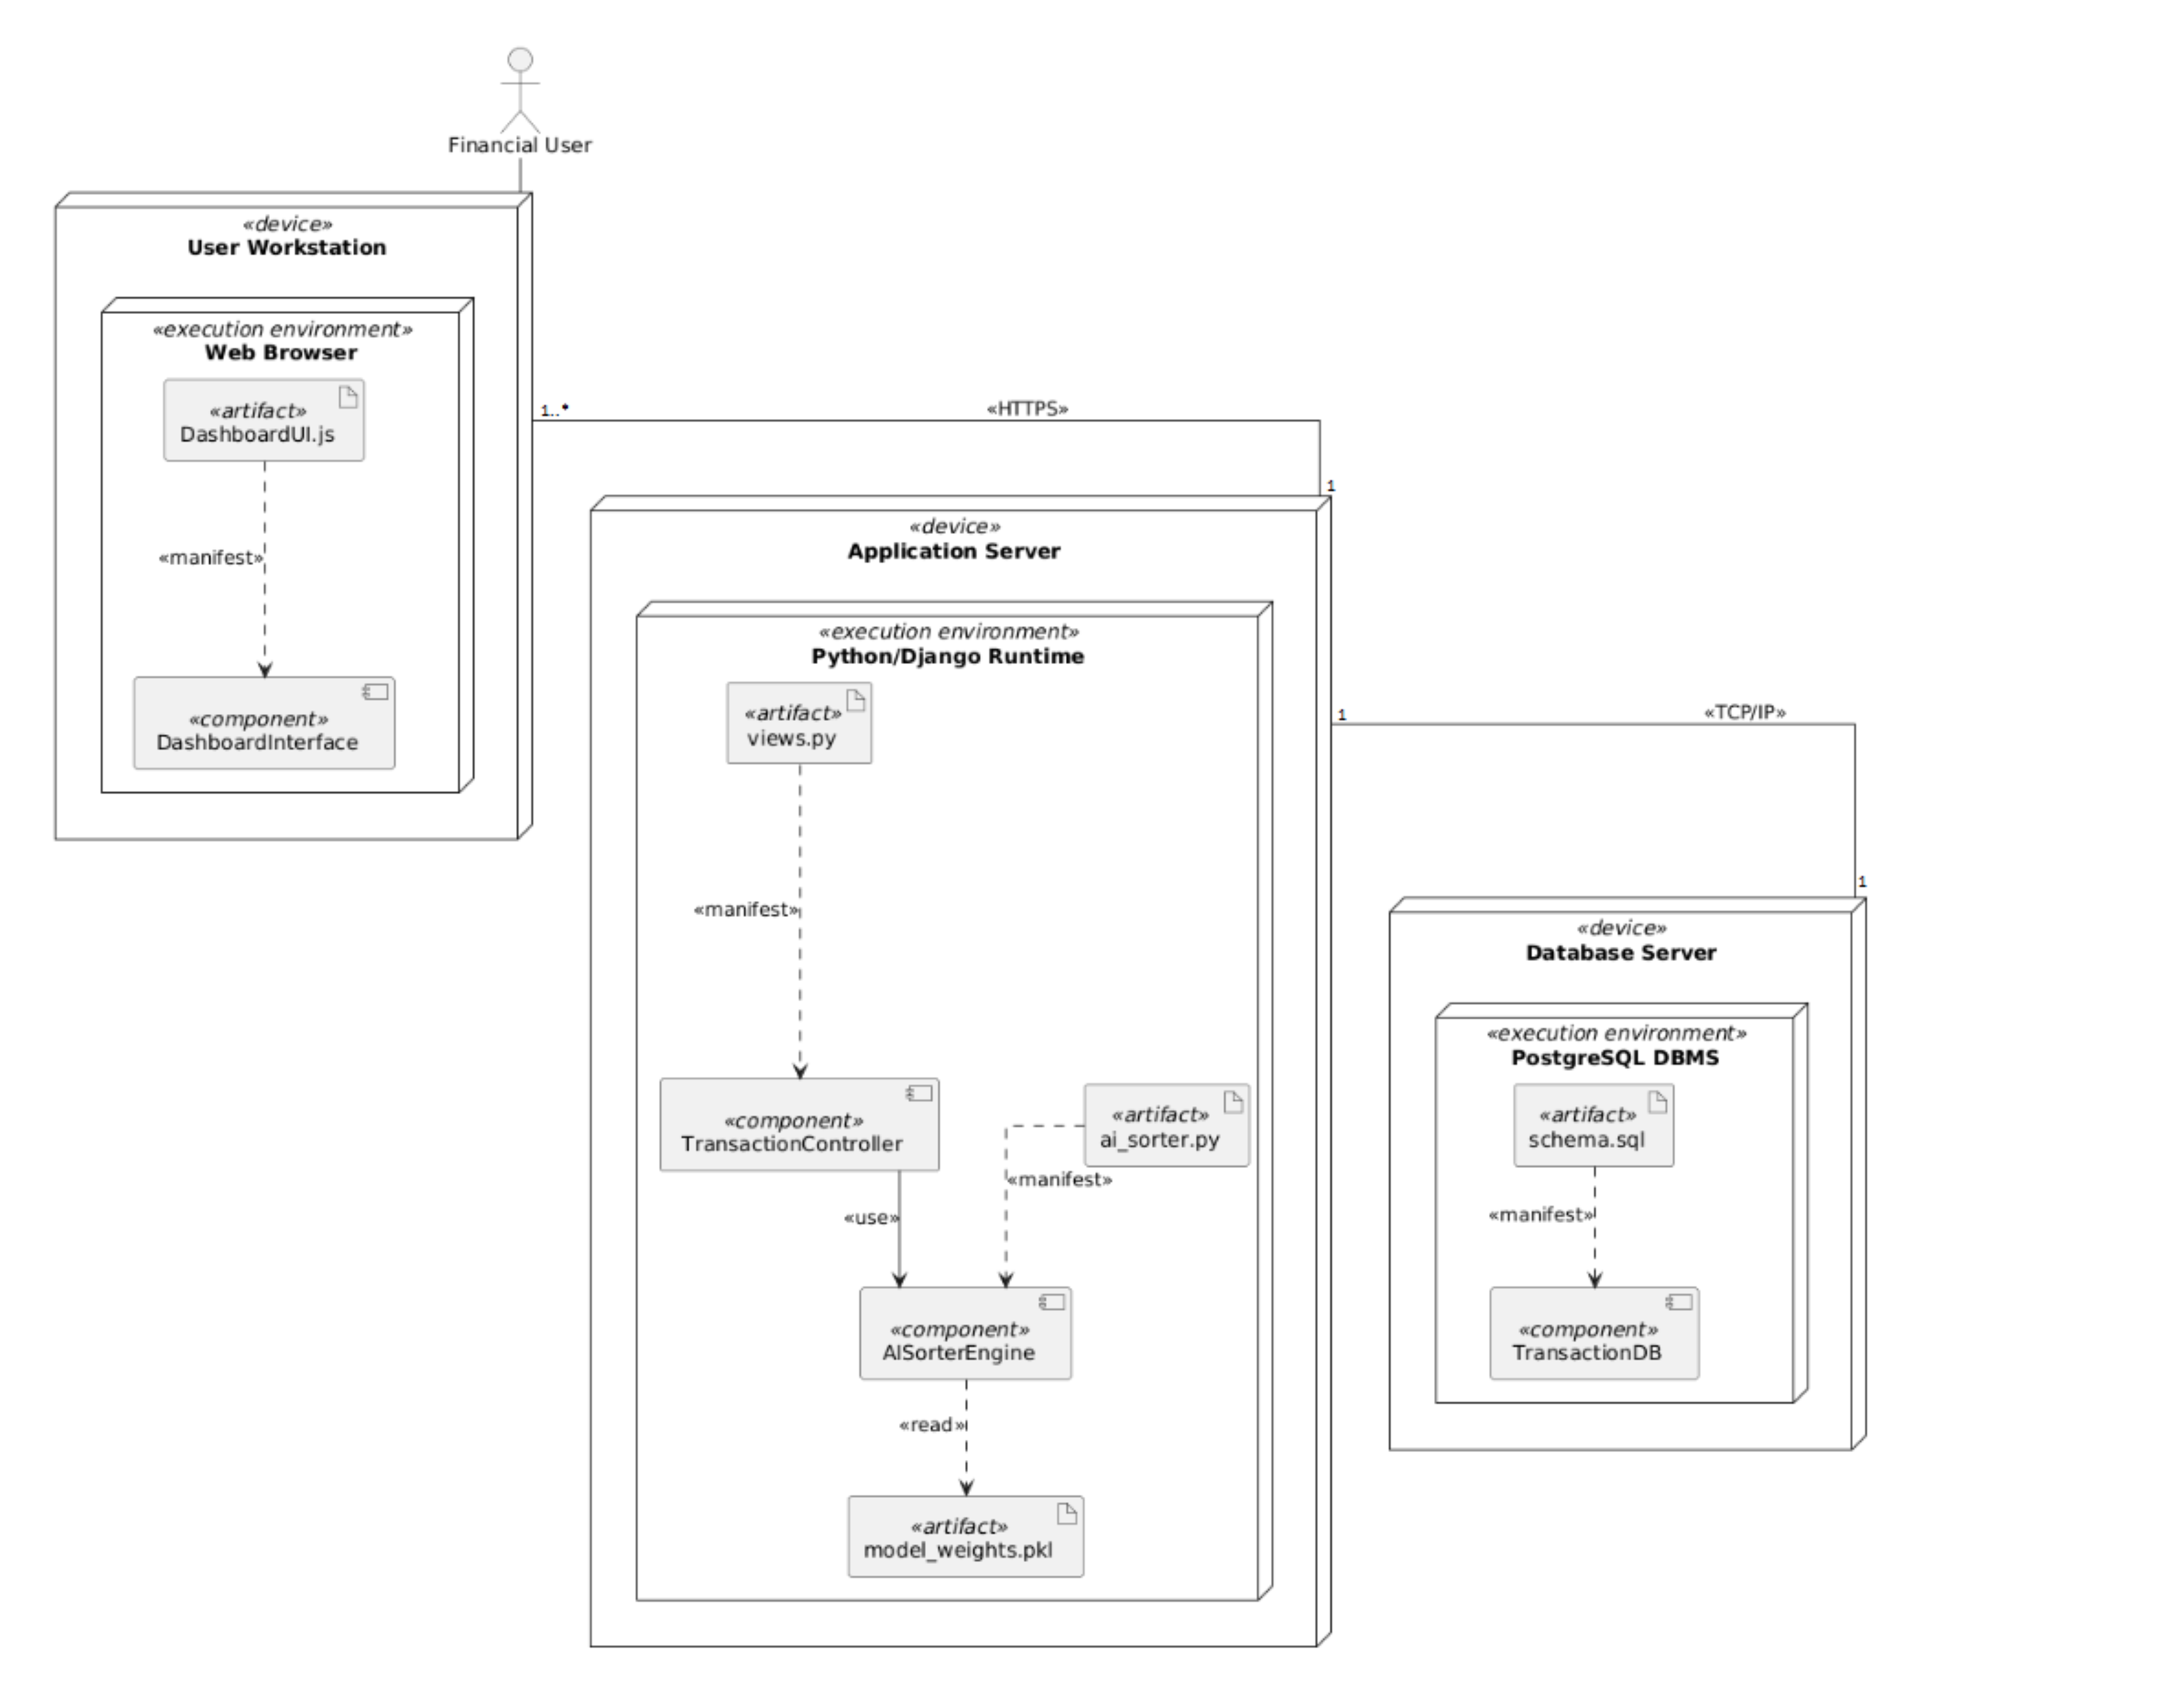
\includegraphics[width=1.0\textwidth, height=0.45\textheight, keepaspectratio]{images/deployment.png}
	\caption{System Deployment Architecture}
	\label{fig:deployment}
\end{figure} % <--- Fixed! No extra '}' here.


\end{document}